\begin{chapterpage}{Introduction to linear regression}
  \chaptertitle{Introduction to linear \titlebreak{} regression}
  \label{linRegrForTwoVar}
  \label{ch_regr_simple_linear}
  \chaptersection{fitting_line_to_data_section}
  \chaptersection{fittingALineByLSR}
  \chaptersection{typesOfOutliersInLinearRegression}
  \chaptersection{inferenceForLinearRegression}
\end{chapterpage}
\renewcommand{\chapterfolder}{ch_regr_simple_linear}
\index{linear regression|textbf}

\chapterintro{Linear regression is a very powerful
  statistical technique.
  Many people have some familiarity with regression just from
  reading the news, where graphs with straight lines are overlaid
  on scatterplots.
  Linear models can be used to see trends and to make predictions.}


\textA{\newpage}

%__________________
\section[Line fitting, residuals, and correlation]{Line fitting, residuals, and correlation }
\label{lineFittingResidualsCorrelation}
\label{fitting_line_to_data_section}

\sectionintro{
\noindent In this section, we examine criteria for identifying a linear model and introduce a new statistic to measure linear \emph{correlation}.  We answer questions such as the following.
\begin{itemize}
\item How do we quantify the strength of the linear association between two numerical variables?
\item What does it mean for two variables to have no association or a nonlinear association?  
\item Once we fit a model, how do we measure the error in the model's predictions?

\end{itemize}

\subsection*{Learning objectives}
\begin{enumerate}
\item Distinguish between the data point y and the predicted value $\hat{y}$ based on a model.

\item Calculate a residual and draw a residual plot.

\item Interpret the standard deviation of the residuals.

\item Interpret the correlation coefficient and estimate it from a scatterplot.

\item Know and apply the properties of the correlation coefficient.
\end{enumerate}
}

%%
\subsection{Beginning with straight lines}

Requests from twelve separate buyers were simultaneously placed with a trading company to purchase Target Corporation stock (ticker \texttt{TGT}, April 26th, 2012).  We let $x$ be the number of stocks to purchase and $y$ be the total cost.  Because the cost is computed using a linear formula, the linear fit is perfect.
\begin{center}
   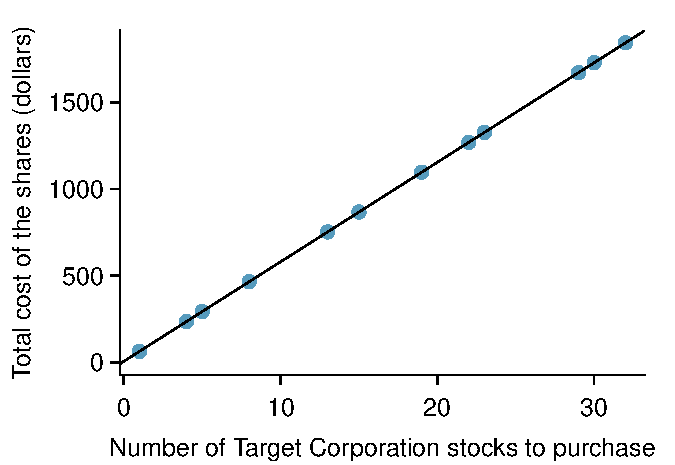
\includegraphics[width=0.5\textwidth]{ch_regr_simple_linear/figures/perfLinearModel/perfLinearModel}
   \label{perfLinearModel}
\end{center}
The equation for the line is: $ y = 5 + 57.49x$

If we know the number of stocks purchased, we can determine the cost based on this linear equation with no error.  Additionally, we can say that each additional share of the stock cost \$57.49 and that there was a \$5 fee for the transaction.


\textA{\newpage}
Perfect linear relationships are unrealistic in almost any natural process. For example, if we took family income $x$, this value would provide some useful information about how much financial support $y$ a college may offer a prospective student. However, family income is only one factor that explains how much financial support a college will offer; there would still be variability in financial support, even when comparing students with the same family income.

When we use $x$ to predict $y$, we usually call $x$ the \term{explanatory variable} or predictor variable, and we call $y$ the \term{response variable}.

In Figure~\ref{imperfLinearModel} we see three scatterplots in which the data fall around a straight line, even if none of the observations fall exactly on the line. The first plot shows a relatively strong downward linear trend, where the remaining variability in the data around the line is minor relative to the strength of the relationship between $x$ and $y$. The second plot shows an upward trend that, while evident, is not as strong as the first. The last plot shows a very weak downward trend in the data, so slight we can hardly notice it. 

In each of these examples, we can consider how to draw a ``best fit line".   For instance, we might wonder, should we move the line up or down a little, or should we tilt it more or less? As we move forward in this chapter, we will learn different criteria for line-fitting, and we will also learn about the uncertainty associated with estimates of model parameters.

\begin{figure}
   \centering
   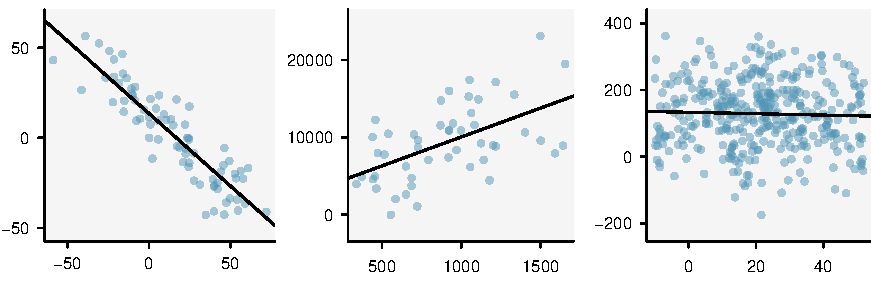
\includegraphics[width=.9\textwidth]{ch_regr_simple_linear/figures/imperfLinearModel/imperfLinearModel}
   \caption{Three data sets where a linear model may be useful even though the data do not all fall exactly on the line.}
   \label{imperfLinearModel}
\end{figure}

We will also see examples in this chapter where fitting a straight line to the data, even if there is a clear relationship between the variables, is not helpful. One such case is shown in Figure~\ref{notGoodAtAllForALinearModel} where there is a very strong relationship between the variables even though the trend is not linear. We will discuss nonlinear trends in this chapter\MultipleRegressionChapter{ and the next}{}, but the details of fitting nonlinear models are saved for a later course.

\begin{figure}
   \centering
   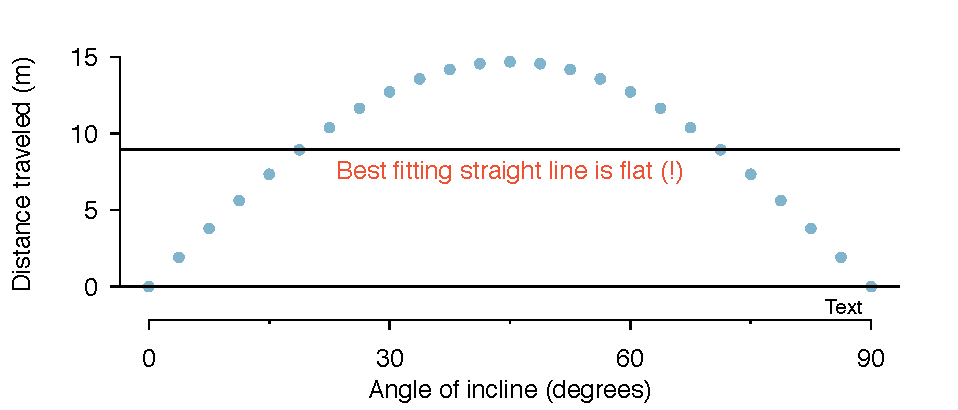
\includegraphics[width=0.6\textwidth]{ch_regr_simple_linear/figures/notGoodAtAllForALinearModel/notGoodAtAllForALinearModel}
   \caption{A linear model is not useful in this nonlinear case. These data are from an introductory physics experiment.}
   \label{notGoodAtAllForALinearModel}
\end{figure}


\index{data!possum|(}

\textA{\newpage}
Scatterplots were introduced in Chapter~\ref{summarizingData} as a graphical technique to present two numerical variables simultaneously. Such plots permit the relationship between the variables to be examined with ease. Figure~\ref{scattHeadLTotalL} shows a scatterplot for the head length and total length of 104 brushtail possums from Australia. Each point represents a single possum from the data.

\begin{figure}
   \centering
\begin{tabular}{cc}

   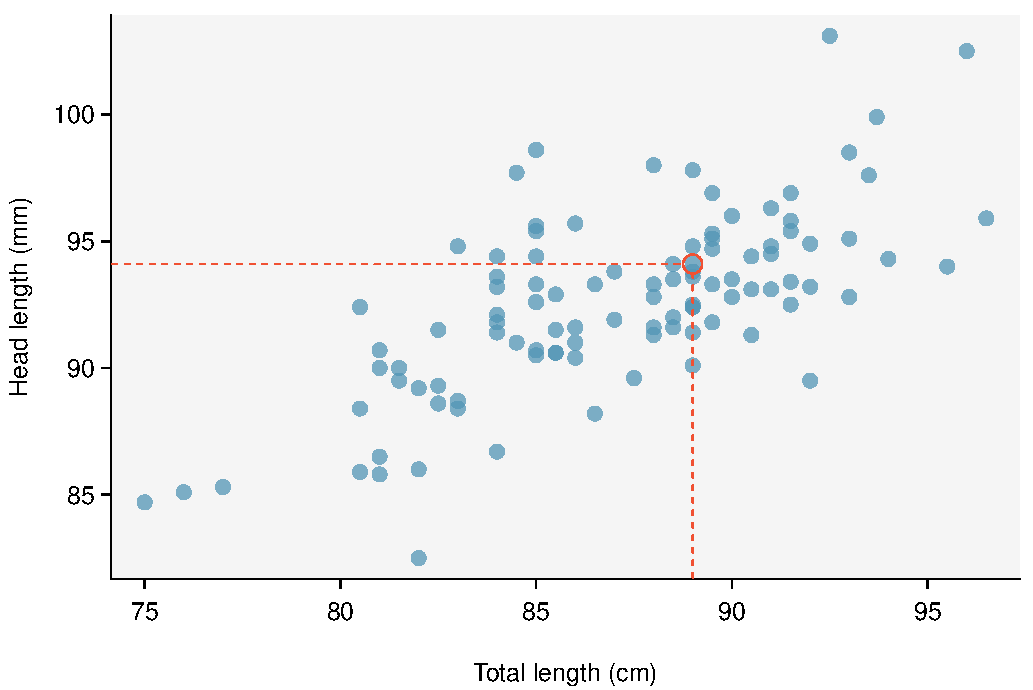
\includegraphics[width=0.7\textwidth]{ch_regr_simple_linear/figures/scattHeadLTotalL/scattHeadLTotalL}
   
\includegraphics[width=0.2\textwidth]{ch_regr_simple_linear/figures/possumPic/possumPic}
\end{tabular}
   \caption{A scatterplot showing head length against total length for 104 brushtail possums. A point representing a possum with head length 94.1mm and total length 89cm is highlighted.}
   \label{scattHeadLTotalL}
\end{figure}
\setlength{\captionwidth}{0.8\mycaptionwidth}

\begin{figure}
   \centering
   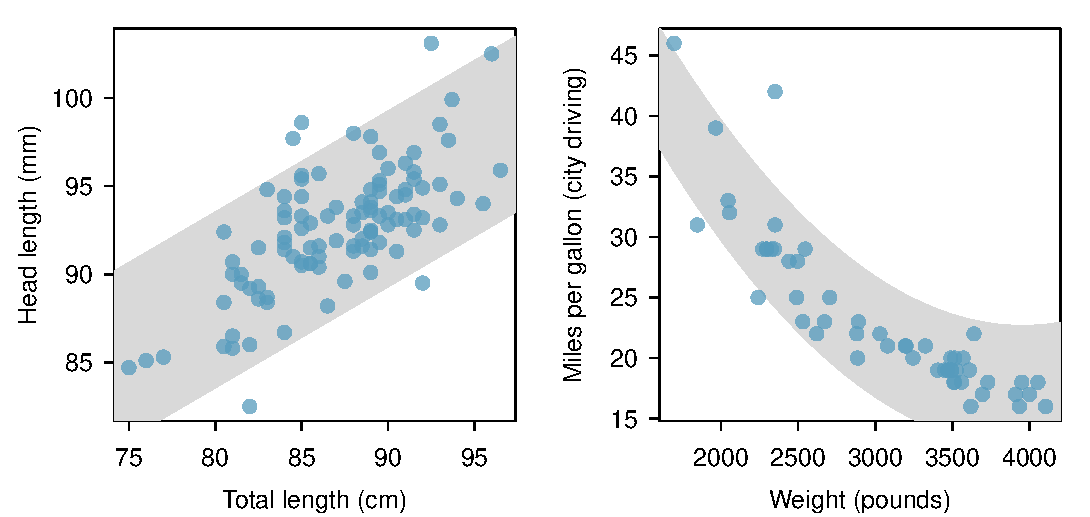
\includegraphics[width=.7\textwidth]{ch_regr_simple_linear/figures/scattHeadLTotalLTube/scattHeadLTotalLTube}
\setlength{\captionwidth}{1\mycaptionwidth}

   \caption{The figure on the left shows head length versus total length, and reveals that many of the points could be captured by a straight band. On the right, we see that a curved band is more appropriate in the scatterplot for \var{weight} and \var{mpgCity} from the \data{cars} data set.}
   \label{scattHeadLTotalLTube}
\end{figure}




The head and total length variables are associated. Possums with an above average total length also tend to have above average head lengths. While the relationship is not perfectly linear, it could be helpful to partially explain the connection between these variables with a straight line.


Straight lines should only be used when the data appear to have a linear relationship, such as the case shown in the left panel of Figure~\ref{scattHeadLTotalLTube}. The right panel of Figure~\ref{scattHeadLTotalLTube} shows a case where a curved line would be more useful in understanding the relationship between the two variables.

\begin{onebox}{Watch out for curved trends}
{We only consider models based on straight lines in this chapter. If data show a nonlinear trend, like that in the right panel of Figure~\ref{scattHeadLTotalLTube}, more advanced techniques should be used.\vspace{0.7mm}}
\end{onebox}

\textA{\newpage}
%%
\Comment{changed subsection title}
\subsection{Predicting based on a line}

We want to describe the relationship between the head length and total length variables in the possum data set using a line. In this example, we will use the total length as the predictor variable, $x$, to predict a possum's head length, $y$. When we use $x$ to predict $y$, we usually call $x$ the \term{explanatory variable} or predictor variable, and we call $y$ the \term{response variable}.  We could fit the linear relationship by eye, as in Figure~\ref{scattHeadLTotalLLine}. The equation for this line is
\begin{eqnarray}
\hat{y} = 41 + 0.59x
\label{headLLinModTotalL}
\end{eqnarray}
We can use this line to discuss properties of possums. For instance, the equation predicts a possum with a total length of 80 cm will have a head length of
\begin{align*}
\hat{y} &= 41 + 0.59(80) \\
	&= 88.2 % mm
\end{align*}
A ``hat'' on $y$ is used to signify that this is a predicted value, not an actual value.  $\hat{y}$ may be viewed as an average: the equation predicts that possums with a total length of 80 cm will have an average head length of 88.2 mm. $\hat{y}$ may also be viewed as a prediction:  Absent further information about an 80 cm possum, this is our best prediction for a the head length of a single 80 cm possum.  



\Comment{rewrote this a little to make simplify}
%%
\subsection{Residuals}
\begin{figure}
   \centering
   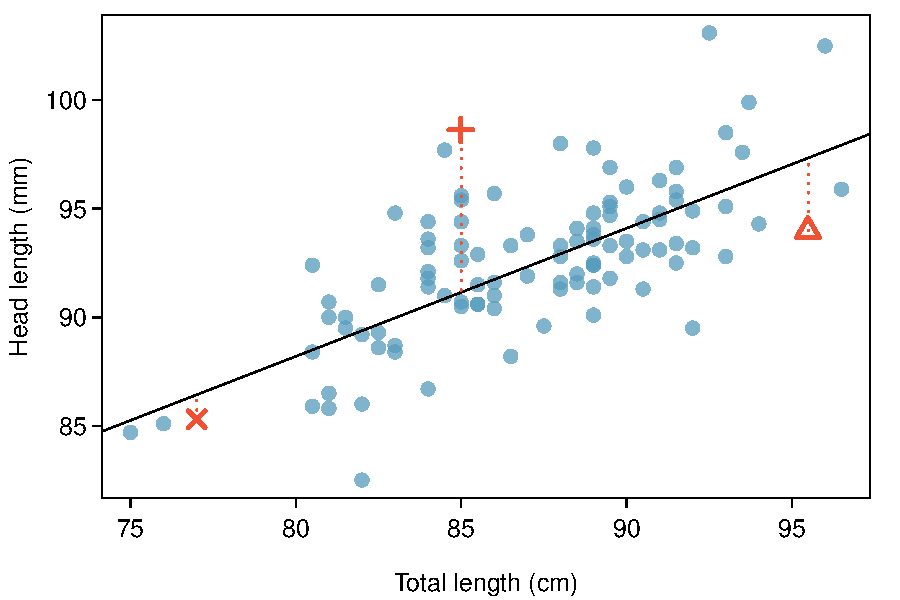
\includegraphics[width=0.8\textwidth]{ch_regr_simple_linear/figures/scattHeadLTotalLLine/scattHeadLTotalLLine}
   \caption{A reasonable linear model was fit to represent the relationship between head length and total length.}
   \label{scattHeadLTotalLLine}
\end{figure}
\index{residual|(}

\termsub{Residuals}{residual} are the leftover variation in the response variable after fitting a model.  Each observation will have a residual.  Looking at Figure~\ref{scattHeadLTotalLLine}, the residual for a particular point is the vertical distance between the point and the line.  This is the distance between the actual value of $y$ and the model prediction for $y$.

If an observation is above the regression line, then its residual is positive.  Observations below the line have negative residuals. One goal in picking the right linear model is for these residuals to be as small as possible.

Three observations are noted specially in Figure~\ref{scattHeadLTotalLLine}. The observation marked by an ``$\times$'' has a small, negative residual of about -1; the observation marked by ``$+$'' has a large residual of about +7; and the observation marked by ``$\triangle$'' has a moderate residual of about -4. The size of a residual is usually discussed in terms of its absolute value. For example, the residual for ``$\triangle$'' is larger than that of ``$\times$'' because $|-4|$ is larger than $|-1|$.

%\Comment{remove use of $e_i$ since students don't need that}



\begin{onebox}{Residual: difference between observed and expected}
The residual for a particular observation $(x, \ y)$ is the difference between the observed response and the response we would predict based on the model:
\begin{align*}
\text{residual} =& \ \text{observed } y - \text{predicted } y\\
 =&\  y - \hat{y}
\end{align*}
We typically identify $\hat{y}$ by plugging $x$ into the model.\end{onebox}

\begin{examplewrap}
\begin{nexample}{The linear fit shown in Figure~\ref{scattHeadLTotalLLine} is given as $\hat{y} = 41 + 0.59x$. Based on this line, compute and interpret the residual of the observation $(77.0, \ 85.3)$. This observation is denoted by ``$\times$'' on the plot. Recall that $x$ is total length measured in cm and $y$ is head length measured in mm.}
We first compute the predicted value based on the model:
\begin{align*}
\hat{y} =& \ 41+0.59x \\
=& \ 41+0.59(77.0)\\
=& \  86.4
\end{align*}
Next we compute the difference of the actual head length and the predicted head length:
\begin{align*}
residual =& \ y - \hat{y} \\
=& \ 85.3 -  86.4 \\
=& \ -1.1
\end{align*}
The residual for this point is -1.1 mm, which is very close to the visual estimate of -1 mm.  For this particular possum with total length of 77 cm, the model's prediction for its head length was 1.1mm \emph{too high}.
\end{nexample}
\end{examplewrap}


\begin{exercisewrap}
\begin{nexercise}
If a model underestimates an observation, will the residual be positive or negative? What about if it overestimates the observation?\footnotemark 
\end{nexercise}
\end{exercisewrap}
\footnotetext{If a model underestimates an observation, then the model estimate is below the actual. The residual, which is the actual observation value minus the model estimate, must then be positive. The opposite is true when the model overestimates the observation: the residual is negative.}

\begin{exercisewrap}
\begin{nexercise}
Compute the residual for the observation $(95.5, 94.0)$ (``$\triangle$'' in the figure) using the linear model: $\hat{y} = 41 + 0.59x$.\footnotemark 
\end{nexercise}
\end{exercisewrap}
\footnotetext{First compute the predicted value based on the model, then compute the residual.
$$\hat{y} = 41+0.59x = 41 + 0.59(95.50) = 97.3$$
$$residual = y - \hat{y} = 94.0 - 97.3 = -3.3$$
The residual is -3.3, so the model \emph{overpredicted} the head length for this possum by 3.3 mm.}
Residuals are helpful in evaluating how well a linear model fits a data set. We often display the residuals in a \term{residual plot} such as the one shown in Figure~\ref{scattHeadLTotalLResidualPlot}.  Here, the residuals are calculated for each $x$ value, and plotted versus $x$.  For instance, the point $(85.0,98.6)$ had a residual of 7.45, so in the residual plot it is placed at $(85.0, 7.45)$. Creating a residual plot is sort of like tipping the scatterplot over so the regression line is horizontal. 

From the residual plot, we can better estimate the \term{standard deviation of the residuals}, often denoted by the letter $s$. %\footnote{This quanitity is also referred to as the standard deviation or standard error about the regression line and is sometimes denote $s_{RES}$, $s_e$ or $s_{\hat{y}}$. The formula is given by $s=\sqrt{\frac{\sum{(y_i-\hat{y})^2}}{n-2}}$, though it need not be memorized.}
The standard deviation of the residuals tells us the average size of the residuals.  As such, it is a measure of the average deviation between the $y$ values and the model predictions.  In other words, it tells us the average prediction error using the model.

\begin{examplewrap}
\begin{nexample}{Estimate the standard deviation of the residuals for predicting head length from total length using the line: $\hat{y} = 41+0.59x$.  Also, interpret the quantity in context.}To estimate this graphically, we use the residual plot.  The approximate 68, 95 rule for standard deviations applies.  Approximately 2/3 of the points are within $\pm$ 2.5 and approximately 95\% of the points are within $\pm$ 5, so 2.5 is a good estimate for the standard deviation of the residuals.  On average, the prediction of head length is off by about 2.5 mm.

\index{data!possum|)}

\end{nexample}
\end{examplewrap}

\begin{onebox}{Standard deviation of the residuals}
The standard deviation of the residuals, often denoted by the letter $s$, tells us the average error in the predictions using the regression model.  It can be estimated from a residual plot.\end{onebox}




\begin{figure}%
   \centering
  \begin{tabular}{cc}
   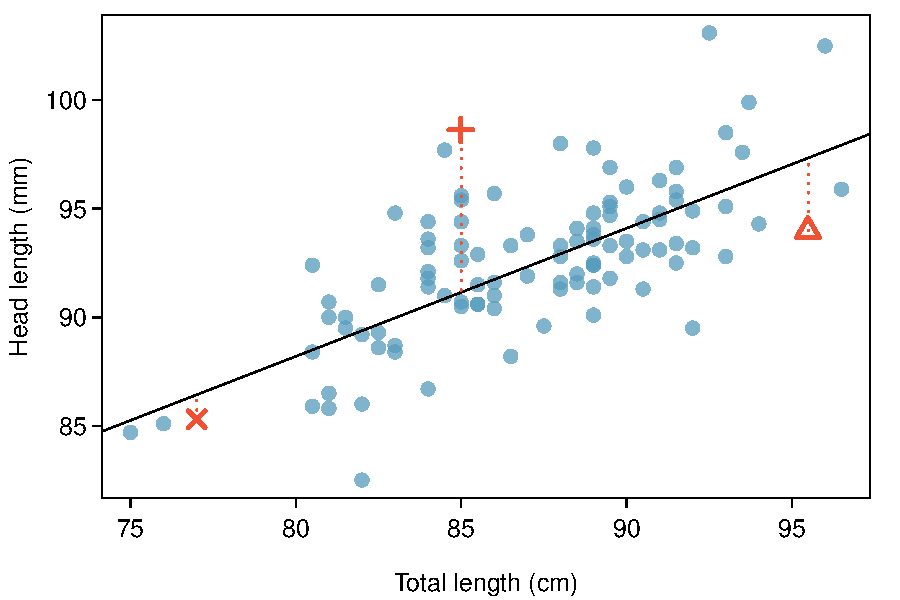
\includegraphics[width=0.5\textwidth]{ch_regr_simple_linear/figures/scattHeadLTotalLLine/scattHeadLTotalLLine}
   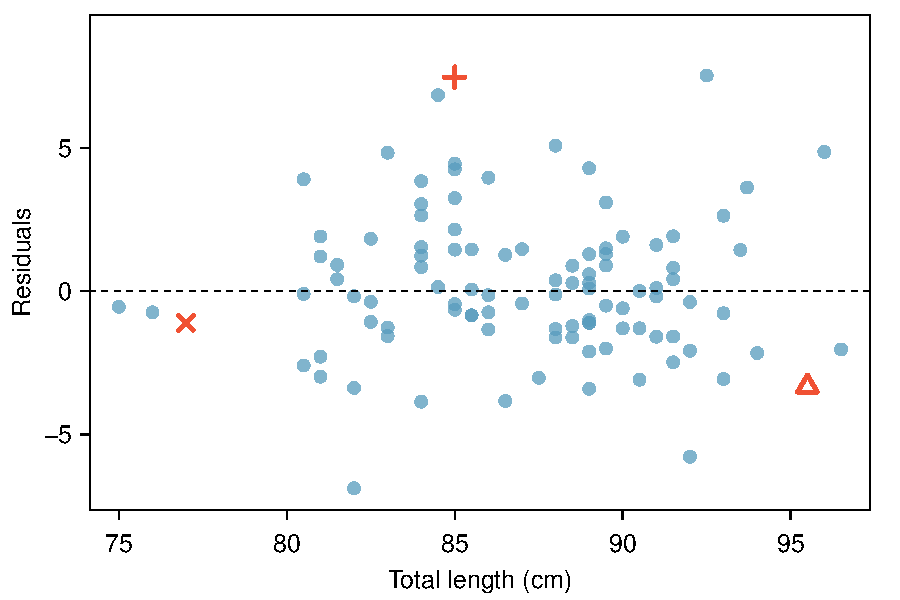
\includegraphics[width=0.5\textwidth]{ch_regr_simple_linear/figures/scattHeadLTotalLResidualPlot/scattHeadLTotalLResidualPlot}
\end{tabular}
\setlength{\captionwidth}{2\mycaptionwidth}
   \caption{Left: Scatterplot with linear model fitted.  \\Right: Residual plot for the model shown in left panel.  }
   \label{scattHeadLTotalLResidualPlot}
\end{figure}

%\Comment{check on placement of figure}

\begin{figure}
   \centering
   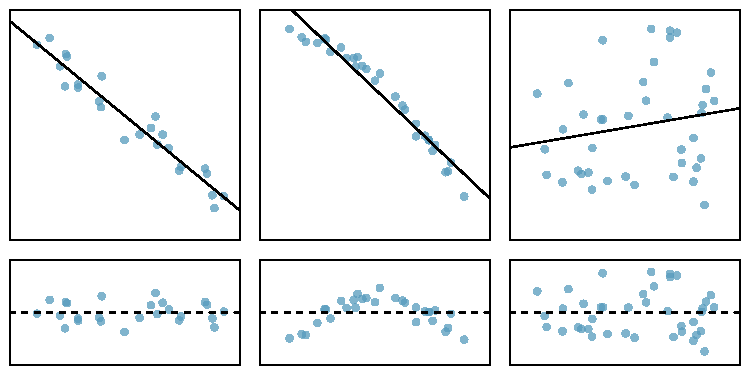
\includegraphics[width=\textwidth]{ch_regr_simple_linear/figures/sampleLinesAndResPlots/sampleLinesAndResPlots}
   \caption{Sample data with their best fitting lines (top row) and their corresponding residual plots (bottom row).}
   \label{sampleLinesAndResPlots}
\end{figure}

\begin{examplewrap}
\begin{nexample}{One purpose of residual plots is to identify characteristics or patterns still apparent in data after fitting a model. Figure~\ref{sampleLinesAndResPlots} shows three scatterplots with linear models in the first row and residual plots in the second row. Can you identify any patterns remaining in the residuals?}


In the first data set (first column), the residuals show no obvious patterns. The residuals appear to be scattered randomly around the dashed line that represents 0.

The second data set shows a pattern in the residuals. There is some curvature in the scatterplot, which is more obvious in the residual plot. We should not use a straight line to model these data. Instead, a more advanced technique should be used.

The last plot shows very little upwards trend, and the residuals also show no obvious patterns. It is reasonable to try to fit a linear model to the data. However, it is unclear whether there is statistically significant evidence that the slope parameter is different from zero. The point estimate of the slope parameter, labeled $b_1$, is not zero, but we might wonder if this could just be due to chance. We will address this sort of scenario in Section~\ref{inferenceForLinearRegression}.
\index{residual|)}
\end{nexample}
\end{examplewrap}



%%
\subsection{Describing linear relationships with correlation}

\index{correlation|(}

\begin{onebox}{Correlation measures the strength of a linear relationship}
\termsub{Correlation}{correlation}, which always takes values between -1 and 1, describes the strength of the linear relationship between two variables. It can be strong, moderate, or~weak.\end{onebox}

We can compute the correlation coefficient, or just correlation for short, using a formula, just as we did with the sample mean and standard deviation. Formally, we can compute the correlation for observations $(x_1, y_1)$, $(x_2, y_2)$, ..., $(x_n, y_n)$ using the formula
\begin{align*}
r =\frac{1}{n-1}\sum{\Big(\frac{x_i-\bar{x}}{s_x}\Big)\Big(\frac{y_i-\bar{y}}{s_y}\Big)}
\end{align*} 
where $\bar{x}$, $\bar{y}$, $s_x$, and $s_y$ are the sample means and standard deviations for each variable. However, this formula is rather complex, so we generally perform the calculations on a computer or calculator. Figure~\ref{posNegCorPlots} shows eight plots and their corresponding correlations. Only when the relationship is perfectly linear is the correlation either -1 or 1. If the relationship is strong and positive, the correlation will be near +1. If it is strong and negative, it will be near -1. If there is no apparent linear relationship between the variables, then the correlation will be near zero.

\begin{figure}
   \centering
   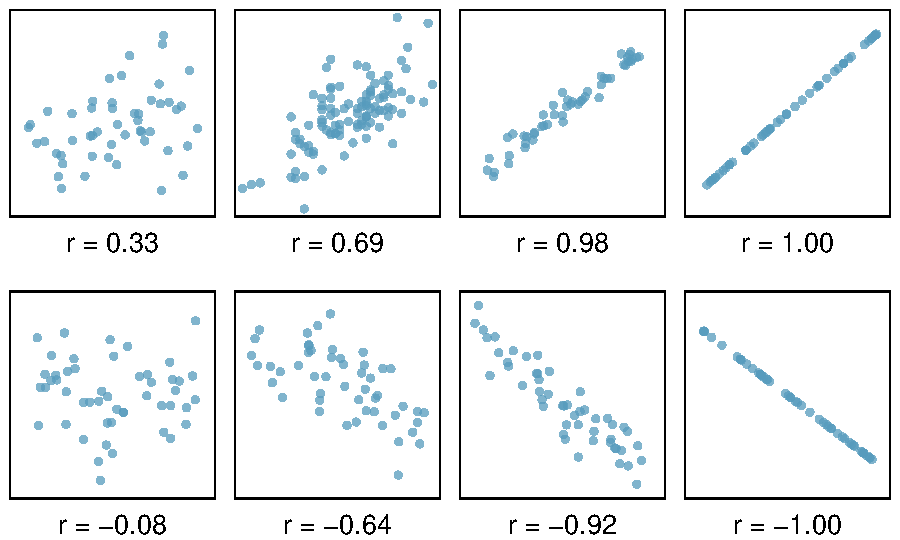
\includegraphics[width=0.95\textwidth]{ch_regr_simple_linear/figures/posNegCorPlots/posNegCorPlots}
   \caption{Sample scatterplots and their correlations. The first row shows variables with a positive relationship, represented by the trend up and to the right. The second row shows variables with a negative trend, where a large value in one variable is associated with a low value in the other.}
   \label{posNegCorPlots}
\end{figure}

The correlation is intended to quantify the strength of a linear trend. Nonlinear trends, even when strong, sometimes produce correlations that do not reflect the strength of the relationship; see three such examples in Figure~\ref{corForNonLinearPlots}.

\begin{figure}
   \centering
   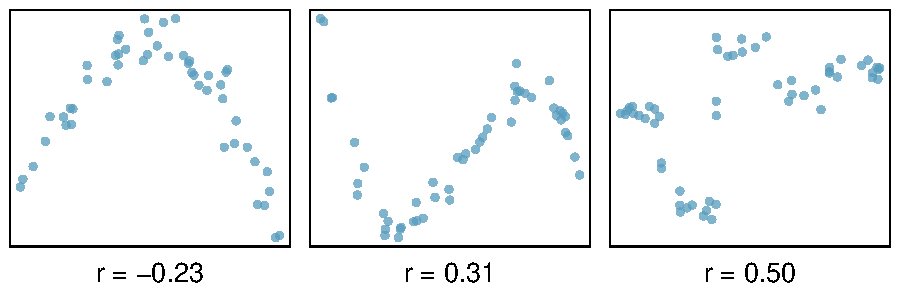
\includegraphics[width=0.96\textwidth]{ch_regr_simple_linear/figures/posNegCorPlots/corForNonLinearPlots}
   \caption{Sample scatterplots and their correlations. In each case, there is a strong relationship between the variables. However, the correlation is not very strong, and the relationship is not linear.}
   \label{corForNonLinearPlots}
\end{figure}

\begin{exercisewrap}
\begin{nexercise}
It appears no straight line would fit any of the datasets represented in Figure~\ref{corForNonLinearPlots}. Try drawing nonlinear curves on each plot. Once you create a curve for each, describe what is important in your fit.\footnotemark 
\index{correlation|)}
\end{nexercise}
\end{exercisewrap}
\footnotetext{We'll leave it to you to draw the lines. In general, the lines you draw should be close to most points and reflect overall trends in the data.}

\begin{examplewrap}
\begin{nexample}
{Take a look at Figure~\ref{scattHeadLTotalLLine} on page~\pageref{scattHeadLTotalLLine}.  How would this correlation change if head length were measured in cm rather than mm?  What if head length were measure in inches rather than mm?}Here, changing the units of $y$ corresponds to multiplying all the $y$ values by a certain number.  This would change the mean and the standard deviation of $y$, but it would not change the correlation.  To see this, imagine dividing every number on the vertical axes by 10.  The units of $y$ are now cm rather than mm, but the graph has remain exactly the same
\end{nexample}
\end{examplewrap}

\begin{onebox}{Changing units of $x$ and $y$ does not affect the correlation.}
The correlation between two variables should not be dependent upon the units in which the variables are recorded.  Adding a constant, subtracting a constant, or multiplying a \emph{positive} constant to all values of $x$ or $y$ does not affect the \mbox{correlation.}\end{onebox}

%%

\textB{\newpage}
%%
\subsection*{Section summary}
\begin{itemize}

\item In Chapter 2 we introduced \term{scatterplots}, which show the relationship between two numerical variables.  When we use $x$ to predict $y$, we call $x$ the \term{explanatory variable} or predictor variable, and we call $y$ the \term{response variable}.

\item A linear model can be useful for prediction when the variables have a constant, linear trend.  Linear models should not be used if the trend between the variables is curved.  

\item $y$ refers to an actual data value.  When we write a linear model, we use $\hat{y}$ to indicate that it is the model or the prediction.   $\hat{y}$ can be understood as a \term{prediction} for $y$ based on a given $x$, or as an \term{average} of the $y$ values for a given $x$.

\item The \term{residual} is the \textbf{error} between the true value and the model, $y - \hat{y}$, for a given $x$-value.  The order of the difference matters, and the sign of the residual will tell us if the model over-predicted or under-predicted a particular data point.

\item The symbol $s$ in a linear model is used to denote the standard deviation of the residuals, and it measures the typical prediction error by the model.

\item A \term{residual plot} is a scatterplot with the residuals on the vertical axis.  The residuals are often plotted against $x$ on the horizontal axis, but they can also be plotted against $y$, $\hat{y}$, or other variables.  Two important uses of a residual plot are the following.
\begin{itemize}
\item Residual plots help us see patterns in the data that may not have been apparent in the scatterplot.
\item The standard deviation of the residuals is easier to estimate from a residual plot than from the original scatterplot.
\end{itemize}

\item The \term{correlation coefficient}, $r$, measures the strength and direction of a linear relationship.  The following are some important properties of $r$.
\begin{itemize}
\item The value of $r$ is always between $-1$ and $1$, inclusive, with an $r=-1$ indicating a perfect negative relationship (points fall exactly along a line that has negative slope) and an $r=1$ indicating a perfect positive relationship (points fall exactly along a line that has positive slope).  
\item An $r=0$ indicates no \emph{linear} association between the variables, though there may well exist a quadratic or other type of association.
\item The calculation of $r$ involves converting the $x$ and $y$ values into Z-scores.  Because of this, changing  the units of $x$ and $y$ does not affect the value of $r$.  Another way to say this is that adding a constant, subtracting a constant, or multiplying a positive constant to all values of $x$ or $y$ does not affect the correlation.
\item Multiplying all values of $x$ or $y$ by a \emph{negative} constant will flip the graph over the $x$ or $y$ axis and therefore change the \emph{sign} of $r$.
\end{itemize}


\end{itemize}


%__________________
\section[Fitting a line by least squares regression]{Fitting a line by least squares regression }
\label{fittingALineByLSR}
\index{least squares regression|(}

\sectionintro{
\begin{itemize}
\item How do we calculate the slope and $y$-intercept of the best fit line?
\item How well can we predict financial aid based on family income for a particular college?
\item How do we measure the fit of a model and compare different models to each other?
\item Why do models sometimes make predictions that are ridiculous or impossible?
\end{itemize}


%%
\subsection*{Learning objectives}
\begin{enumerate}
\item Calculate the slope and y-intercept of the least squares regression line using the relevant summary statistics.  Interpret these quantities in context.

\item Understand why the least squares regression line is called the least squares regression line.

\item Interpret the explained variance $R^2$.

\item Understand when extrapolation is occuring and why that is dangerous.

\item Identify outliers and influential points in a scatterplot.

\end{enumerate}
}


%%
\subsection{An objective measure for finding the best line}
Fitting linear models by eye is open to criticism since it is based on an individual preference. In this section, we use \emph{least squares regression} as a more rigorous approach.

This section considers family income and gift aid data from a random sample of fifty students in the 2011 freshman class of Elmhurst College in Illinois.\footnote{These data were sampled from a table of data for all freshman from the 2011 class at Elmhurst College that accompanied an article titled \emph{What Students Really Pay to Go to College} published online by \emph{The~Chronicle of Higher Education}: \oiRedirect{textbook-chronicle_elmhurst_article}{chronicle.com/article/What-Students-Really-Pay-to-Go/131435}} Gift aid is financial aid that does not need to be paid back, as opposed to a loan. A scatterplot of the data is shown in Figure~\ref{elmhurstScatterW2Lines} along with two linear fits. The lines follow a negative trend in the data; students who have higher family incomes tended to have lower gift aid from the university.

\begin{figure}
\centering
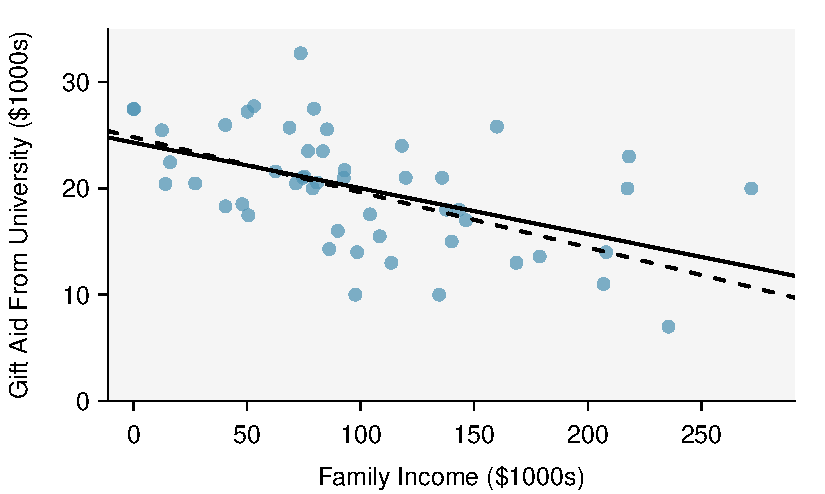
\includegraphics[width=0.75\textwidth]{ch_regr_simple_linear/figures/elmhurstPlots/elmhurstScatterW2Lines}
\caption{Gift aid and family income for a random sample of 50 freshman students from Elmhurst College. Two lines are fit to the data, the solid line being the \emph{least squares line}.}
\label{elmhurstScatterW2Lines}
\end{figure}


We begin by thinking about what we mean by ``best''. Mathematically, we want a line that has small residuals. Perhaps our criterion could minimize the sum of the residual magnitudes:
\begin{eqnarray*}
|y_1 - \hat{y}_1| + |y_2-\hat{y}_2| + \dots + |y_n-\hat{y}_n|
\label{sumOfAbsoluteValueOfResiduals}
\end{eqnarray*}
which we could accomplish with a computer program. The resulting dashed line shown in Figure~\ref{elmhurstScatterW2Lines} demonstrates this fit can be quite reasonable. However, a more common practice is to choose the line that minimizes the sum of the squared residuals:
\begin{eqnarray*}
(y_1 - \hat{y}_1)^2 + (y_2-\hat{y}_2)^2+ \dots + (y_n-\hat{y}_n)^2
\label{sumOfSquaresForResiduals}
\end{eqnarray*}
The line that minimizes the sum of the squared residuals is represented as the solid line in Figure~\ref{elmhurstScatterW2Lines}. This is commonly called the \term{least squares line}. 

Both lines seem reasonable.  Why do statisticians prefer the least squares regression line?  One reason is that it is easier to compute by hand and in most statistical software.  Another, and more compelling, reason is that in many applications, a residual twice as large as another residual is more than twice as bad. For example, being off by 4 is usually more than twice as bad as being off by 2. Squaring the residuals accounts for this discrepancy.

%%
\subsection{Finding the least squares line}
\label{findingTheLeastSquaresLineSection}

For the Elmhurst data, we could fit a least squares regression line for predicting gift aid based on a student's family income and write the equation as:
\begin{eqnarray*}
\widehat{aid} = b_0 + b_1\times family\_\hspace{0.3mm}income
\end{eqnarray*}
Here $b_0$ is the $y$-intercept of the least squares regression line and $b_1$ is the slope of the least squares regression line.  $b_0$ and $b_1$ are both statistics that can be calculated from the data.  In the next section we will consider the corresponding parameters that they statistics attempt to estimate.  

We can enter all of the data into a statistical software package and easily find the values of $b_0$ and $b_1$.  However, we can also calculate these values by hand, using only the summary statistics.
\begin{itemize}
\item The slope of the least squares line is given by
\begin{eqnarray*}
b_1 = r\frac{s_y}{s_x}
\label{slopeOfLSRLine}
\end{eqnarray*}
where $r$ is the correlation between the variables $x$ and $y$, and $s_x$ and $s_y$ are the sample standard deviations of $x$, the explanatory variable, and $y$, the response variable.
\item The point of averages $(\bar{x}, \bar{y})$ is always on the least squares line. Plugging this point in for $x$ and $y$ in the least squares equation and solving for $b_0$ gives
\begin{align*}
\bar{y} &= b_0 + b_1\bar{x}
&&b_0=\bar{y}-b_1\bar{x}
\label{interceptOfLSRLine}
\end{align*}
\end{itemize}


\begin{onebox}{Finding the slope and intercept of the least squares regression line}
The least squares regression line for predicting $y$ based on $x$ can be written as:  $\hat{y}=b_0+b_1x$.  
\begin{align*}
b_1=r\frac{s_y}{s_x} \\
b_0=\bar{y}-b_1\bar{x}
\end{align*}
We first find $b_1$, the slope, and then we solve for $b_0$, the $y$-intercept.  
\end{onebox}

\begin{exercisewrap}
\begin{nexercise}
Table~\ref{summaryStatsOfSATGPAData} shows the sample means for the family income and gift aid as \$101,800 and \$19,940, respectively. Plot the point $(101.8, 19.94)$ on Figure~\vref{elmhurstScatterW2Lines} to verify it falls on the least squares line (the solid line).\footnotemark 
\end{nexercise}
\end{exercisewrap}
\footnotetext{If you need help finding this location, draw a straight line up from the x-value of 100 (or thereabout). Then draw a horizontal line at 20 (or thereabout). These lines should intersect on the least squares line.}

\begin{table}[ht]
\centering
\begin{tabular}{l rr}
\hline
\vspace{-4mm} & & \\
\vspace{0.4mm}	&	\ \ family income, in \$1000s (``$x$'')	& \ \ gift aid, in \$1000s (``$y$'') \\
\hline
  \vspace{-3.9mm} & & \\
mean	& $\bar{x} = 101.8$		& $\bar{y} = 19.94$ \\
sd		& $s_x = 63.2$		& $s_y = 5.46$\vspace{0.4mm} \\
\hline
\vspace{-4mm}\ &\\
	& \multicolumn{2}{r}{$r=-0.499$} \\
\hline
\end{tabular}
\caption{Summary statistics for family income and gift aid.}
\label{summaryStatsOfSATGPAData}
\end{table}

\begin{examplewrap}
\begin{nexample} 
{Using the summary statistics in Table~\ref{summaryStatsOfSATGPAData}, find the equation of the least squares regression line for predicting gift aid based on family income.}
\begin{align*}
b_1 &= r\frac{s_y}{s_x} = (-0.499)\frac{5.46}{63.2} = -0.0431 \\
b_0 & = \bar{y} - b_1\bar{x} = 101.8 - (-0.0431)(19.94) = 24.3\\
\\
\hat{y}&=24.3 - 0.0431x
	\qquad\text{or}\qquad
	\widehat{aid} = 24.3 - 0.0431\times family\_\hspace{0.3mm}income
\end{align*}
\end{nexample}
\end{examplewrap}
\label{findingTheSlopeOfTheLSRLineForIncomeAndAid}

\begin{examplewrap}
\begin{nexample}{Say we wanted to predict a student's family income based on the amount of gift aid that they received.  Would this least squares regression line be:
$aid = 24.3 - 0.0431\times \widehat{family\_\hspace{0.3mm}income}$?}
No.  The equation we found was for predicting aid, not for predicting family income.  We would have to calculate a new regression line, letting $y$ be $family\_\hspace{0.3mm}income$ and $x$ be $aid$.  This would give us:
\begin{align*}
b_1 &= r\frac{s_y}{s_x} = (-0.499)\frac{63.2}{5.46} = -5.776 \\
b_0 & = \bar{y} - b_1\bar{x} = 19.94 - (-5.776)(101.8) = 607.9\\
\\
\hat{y}&=607.3 - 5.776x
	\qquad\text{or}\qquad
	\widehat{family\_\hspace{0.3mm}income} = 607.3 - 5.776\times aid
\end{align*}

\end{nexample}
\end{examplewrap} 


We mentioned earlier that a computer is usually used to compute the least squares line. A summary table based on computer output is shown in Table~\ref{rOutputForIncomeAidLSRLine} for the Elmhurst data. The first column of numbers provides estimates for ${b}_0$ and ${b}_1$, respectively. Compare these to the result from Exercise~\ref{findingTheSlopeOfTheLSRLineForIncomeAndAid}.

\begin{table}[ht]
\centering
\begin{tabular}{l rrrr}
  \hline
  \vspace{-3.7mm} & & & & \\
 & Estimate & Std. Error & t value & Pr($>$$|$t$|$) \\ 
  \hline
  \vspace{-3.6mm} & & & & \\
(Intercept) & 24.3193 & 1.2915 & 18.83 & 0.0000 \\ 
family\_\hspace{0.3mm}income & -0.0431 & 0.0108 & -3.98 & 0.0002 \\ 
  \hline
\end{tabular}
\caption{Summary of least squares fit for the Elmhurst data. Compare the parameter estimates in the first column to the results of Guided Practice~\ref{findingTheSlopeOfTheLSRLineForIncomeAndAid}.}
\label{rOutputForIncomeAidLSRLine}
\end{table}

\begin{examplewrap}
\begin{nexample}{Examine the second, third, and fourth columns in Table~\ref{rOutputForIncomeAidLSRLine}. Can you guess what they represent?}
We'll look at the second row, which corresponds to the slope.  The first column, Estimate, tells us our best estimate for the true slope.  We call this point estimate $b_1$.  The second column is the standard error of this point estimate: 0.0108. The third column is a $T$ test statistic for the null hypothesis that $\beta_1 = 0$: $T=-3.98$. The last column is the p-value for the $T$ test statistic for the null hypothesis $\beta_1=0$ and a two-sided alternative hypothesis: 0.0002. We will get into more of these details in Section~\ref{inferenceForLinearRegression}.
\end{nexample}
\end{examplewrap}

\begin{examplewrap}
\begin{nexample}{Suppose a high school senior is considering Elmhurst College. Can she simply use the linear equation that we have found to calculate her financial aid from the university?}
No.  Using the equation will provide a prediction or estimate.  However, as we see in the scatterplot, there is a lot of variability around the line.  While the linear equation is good at capturing the trend in the data, there will be significant error in predicting an individual student's aid.  Additionally, the data all come from one freshman class, and the way aid is determined by the university may change from year to year.
\end{nexample}
\end{examplewrap} 


%%
\subsection{Interpreting the coefficients of a regression line}

\index{least squares regression!interpreting parameters|(}

Interpreting the coefficients in a regression model is often one of the most important steps in the analysis.

\begin{examplewrap}
\begin{nexample}{The slope for the Elmhurst data for predicting gift aid based on family income was calculated as -0.0431.  Intepret this quantity in the context of the problem.   and 24.3, respectively.  }
Slope represents a change in $y$ over a change in $x$.  The units for slope are (units of $y$)/(units of $x$).  Here, both $x$ and $y$ are in thousands of dollars.  We can think of -0.0431 as -0.0431/1.  The slope, then, tells us that when $x$ goes up by 1, on average, $y$ goes down by 0.0431.  In other words, for each additional thousand dollars of family income, \emph{on average}, students receive 0.0431 thousand, or \$43.10 \emph{less} in gift aid. Note that a higher family income corresponds to less aid because the slope is negative.   
\end{nexample}
\end{examplewrap}

\begin{examplewrap}
\begin{nexample}{The $y$-intercept for the Elmhurst data for predicting gift aid based on family income was calculated as 24.3.  Intepret this quantity in the context of the problem. }
The intercept $b_0$ describes the predicted value of $y$ when $x=0$.  The \emph{predicted} gift aid is 24.3 thousand dollars if a student's family has no income.  The meaning of the intercept is relevant to this application since the family income for some students at Elmhurst is \$0. In other applications, the intercept may have little or no practical value if there are no observations where $x$ is near zero.  Here, it would be acceptable to say that the \emph{average} gift aid is 24.3 thousand dollars among students whose family have 0 dollars in income.
\end{nexample}
\end{examplewrap}

\begin{onebox}{Interpreting coefficients in a linear model}
\vspace{-4mm}
\begin{itemize}
\setlength{\itemsep}{0mm}
\item The slope, $b_1$, describes the \emph{average} increase or decrease in the $y$ variable if the explanatory variable $x$ is one unit larger. 
\item The y-intercept, $b_0$, describes the predicted outcome of $y$ if $x=0$.  The linear model must be valid all the way to $x=0$ for this to make sense, which in many applications is not the case.
\end{itemize}
\end{onebox}

\index{least squares regression!interpreting parameters|)}

\begin{exercisewrap}
\begin{nexercise}
In the previous chapter, we encountered a data set that compared the price of new textbooks for UCLA courses at the UCLA Bookstore and on Amazon.  We fit a linear model for predicting price at UCLA Bookstore from price on Amazon and we get:  
\begin{align*}
\hat{y} = 1.86 + 1.03x
\end{align*}
where $x$ is the price on Amazon and $y$ is the price at the UCLA bookstore.  Interpret the coefficients in this model and discuss whether the interpretations make sense in this context.\footnotemark
\end{nexercise}
\end{exercisewrap}
\footnotetext{The $y$-intercept is 1.86 and the units of $y$ are in dollars.  This tells us that when a textbook costs 0 dollars on Amazon, the predicted price of the textbook at the UCLA Bookstore is 1.86 dollars.  This does not make sense as Amazon does not sell any \$0 textbooks.  The slope is 1.03, with units (dollars)/(dollars).  On average, for every extra dollar that a book costs on Amazon, it costs an extra 1.03 dollars at the UCLA Bookstore.  This interpretation does make sense in this context.
}


\begin{exercisewrap}
\begin{nexercise}
Can we conclude that if Amazon raises the price of a textbook by 1 dollar, the UCLA Bookstore will raise the price of the textbook by \$1.03?\footnotemark
\end{nexercise}
\end{exercisewrap}
\footnotetext{No.  The slope describes the overall trend.  This is observational data; a causal conclusion cannot be drawn.  Remember, a causal relationship can only be concluded by a well designed randomized, controlled experiment.  Additionally, there may be large variation in the points about the line.  The slope does not tell us how much $y$ might change based on a change in $x$ for a particular textbook.
}

\begin{onebox}{Exercise caution when interpreting coefficients of a linear model}
\vspace{-4mm}
\begin{itemize}
\setlength{\itemsep}{0mm}
\item The slope tells us only the \emph{average} change in $y$ for each unit change in $x$; it does not tell us how much $y$ might change based on a change in $x$ for any particular \emph{individual}.  Moreover, in most cases, the slope cannot be interpreted in a causal way.
\item If there are no data points near $x=0$, then the $y$-intercept of the model may be inaccurate, impossible, or ridiculous.  
\end{itemize}
\end{onebox}



%%
\subsection{Extrapolation is treacherous}

\index{least squares regression!extrapolation|(}

{\em\small When those blizzards hit the East Coast this winter, it proved to my satisfaction that global warming was a fraud. That snow was freezing cold. But in an alarming trend, temperatures this spring have risen. Consider this: On February $6^{th}$ it was 10 degrees. Today it hit almost 80. At this rate, by August it will be 220 degrees. So clearly folks the climate debate rages on.\vspace{0.5mm}}

\noindent\hspace{\textwidth}\hspace{-40mm}Stephen Colbert

\noindent\hspace{\textwidth}\hspace{-40mm}April 6th, 2010 \footnote{\oiRedirect{textbook-colbert_extrapolation}{www.cc.com/video-clips/l4nkoq/}} \\

Linear models can be used to approximate the relationship between two variables. However, these models have real limitations. Linear regression is simply a modeling framework. The truth is almost always much more complex than our simple line. For example, we do not know how the data outside of our limited window will behave.

\begin{examplewrap}
\begin{nexample}{Use the model $\widehat{aid} = 24.3 - 0.0431\times family\_\hspace{0.3mm}income$ to estimate the aid of another freshman student whose family had income of \$1 million.}
Recall that the units of family income are in \$1000s, so we want to calculate the aid for $family\_\hspace{0.3mm}income = 1000$:
\begin{align*}
\widehat{aid} &= 24.3 - 0.0431 \times family\_\hspace{0.3mm}income \\
\widehat{aid}&=24.3 - 0.431(1000) = -18.8
\end{align*}
The model predicts this student will have -\$18,800 in aid (!). Elmhurst College cannot (or at least does not) require any students to pay extra on top of tuition to attend.
\end{nexample}
\end{examplewrap}

Applying a model estimate to values outside of the realm of the original data is called \term{extrapolation}. Generally, a linear model is only an approximation of the real relationship between two variables. If we extrapolate, we are making an unreliable bet that the approximate linear relationship will be valid in places where it has not been analyzed.

\index{least squares regression!extrapolation|)}



%%
\subsection{Using $R^2$ to describe the strength of a fit}

\index{least squares regression!R-squared ($R^2$)|(}

We evaluated the strength of the linear relationship between two variables earlier using the correlation coefficient, $r$. However, it is more common to explain the strength of a linear fit using $R^2$, called \termsub{R-squared}{least squares regression!R-squared ($R^2$)} or the \term{explained variance}. If provided with a linear model, we might like to describe how closely the data cluster around the linear fit.

\Comment{TODO(David) Can you add a dashed horizontal line at ybar, and draw a dashed or dotted vertical line from one of the points to ybar and from that same point to yhat - to illustrate how to understand $r^2$?  See R$\_$sqGraphic.png on AP Statistics dropbox for an example.}

\begin{figure}
\centering
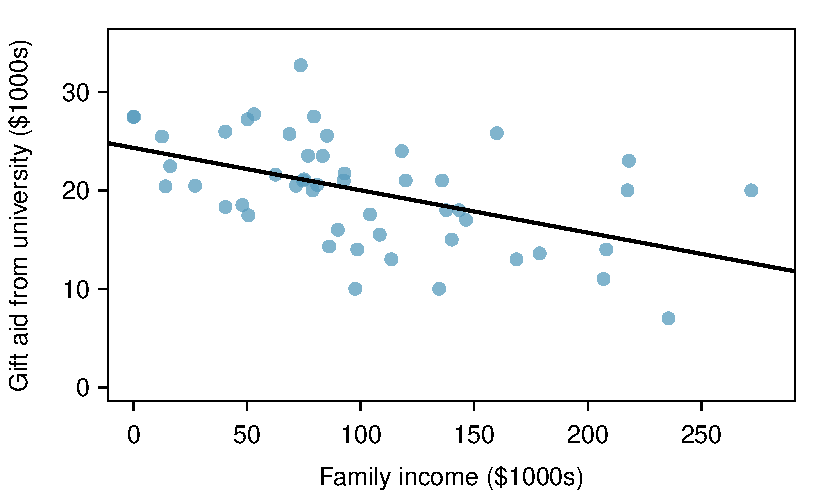
\includegraphics[width=0.75\textwidth]{ch_regr_simple_linear/figures/elmhurstPlots/elmhurstScatterWLSROnly}
\caption{Gift aid and family income for a random sample of 50 freshman students from Elmhurst College, shown with the least squares regression line.}
\label{elmhurstScatterWLSROnly}
\end{figure}

The $R^2$ of a linear model describes the amount of variation in the response that is explained by the least squares line. For example, consider the Elmhurst data, shown in Figure~\ref{elmhurstScatterWLSROnly}. The variance of the response variable, aid received, is $s_{aid}^2=29.8$. However, if we apply our least squares line, then this model reduces our uncertainty in predicting aid using a student's family income. The variability in the residuals describes how much variation remains after using the model: $s_{_{RES}}^2 = 22.4$.  In short, there was a reduction of
$$\frac{s_{aid}^2 - s_{_{RES}}^2}{s_{aid}^2}
	= \frac{29.8 - 22.4}{29.8} = \frac{7.5}{29.8}
	= 0.25$$
This is how we compute the $R^2$ value.\footnote{$R^2=1-\frac{s^2_{RES}}{s^2_y}$} It also corresponds to the square of the correlation coefficient, $r$, that~is, $R^2=r^2$.
\begin{align*}
R^2 &= 0.25 & r &= -0.499
\end{align*}

\begin{onebox}{$R^2$ is the explained variance}
$R^2$ is always between 0 and 1, inclusive.  It tells us the proportion of variation in the $y$ values that is explained by a regression model.  The higher the value of $R^2$, the better the model ``explains" the response variable.
\end{onebox}

\begin{exercisewrap}
\begin{nexercise}
If a linear model has a very strong negative relationship with a correlation of -0.97, how much of the variation in the response variable is explained by the explanatory variable?\footnotemark 
\end{nexercise}
\end{exercisewrap}
\footnotetext{About $R^2 = (-0.97)^2 = 0.94$ or 94\% of the variation in aid is explained by the linear model.}
\index{least squares regression!R-squared ($R^2$)|)}

\begin{exercisewrap}
\begin{nexercise}
If a linear model has an $R^2$ or explained variance of 0.94, what is the correlation coefficient?\footnotemark 
\end{nexercise}
\end{exercisewrap}
\footnotetext{We take the square root of $R^2$ and get 0.97, but we must be careful, because $r$ could be 0.97 \emph{or} -0.97.  Without knowing the slope or seeing the scatterplot, we have no way of knowing if $r$ is positive or negative.}

%%
\subsection{Calculator: linear correlation and regression}
\label{calclinreg}

\begin{onebox}{\videohref{ti84_calculating_regression_summary_statistics} TI-84: finding $b_0$, $b_1$, $R^2$, and $r$ for a linear model}
Use \calctext{STAT}, \calctext{CALC}, \calctext{LinReg(a + bx)}.
\begin{enumerate}
\setlength{\itemsep}{0mm}
\item Choose \calctext{STAT}.
\item Right arrow to \calctext{CALC}.
\item Down arrow and choose \calctext{8:LinReg(a+bx)}.\vspace{-1.5mm}
  \begin{itemize}
  \item Caution: choosing \calctext{4:LinReg(ax+b)} will reverse $a$ and $b$.
  \end{itemize}
\item Let \calctext{Xlist} be \calctext{L1} and \calctext{Ylist} be \calctext{L2} (don't forget to enter the $x$ and $y$ values in L1 and \calctext{L2} before doing this calculation).  
\item Leave \calctext{FreqList} blank.
\item Leave \calctext{Store RegEQ} blank.
\item Choose Calculate and hit \calctext{ENTER}, which returns: \\[1mm]
\begin{tabular}{l l}
\calctext{a} & $b_0$, the y-intercept of the best fit line \\
\calctext{b} & $b_1$, the slope of the best fit line \\
$\calctextmath{r^2}$ & $R^2$, the explained variance \\
\calctext{r} & $r$, the correlation coefficient
\end{tabular}
\end{enumerate}
TI-83: Do steps 1-3, then enter the $x$ list and $y$ list separated by a comma, e.g. \calctext{LinReg(a+bx) L1, L2}, then hit \calctext{ENTER}.\end{onebox} 

\begin{onebox}{What to do if $r^2$ and $r$ do not show up on a TI-83/84}
If $r^2$ and $r$ do now show up when doing \calctext{STAT}, \calctext{CALC}, \calctext{LinReg}, the \emph{diagnostics} must be turned on.  This only needs to be once and the diagnostics will remain on.
\begin{enumerate}
\setlength{\itemsep}{0mm}
\item Hit \calctext{2ND} \calctext{0} (i.e. \calctext{CATALOG}).
\item Scroll down until the arrow points at \calctext{DiagnosticOn}.
\item Hit \calctext{ENTER} and \calctext{ENTER} again. The screen should now say: \\[1mm]
\begin{tabular}{l l}
\calctext{DiagnosticOn} & \\
& \calctext{Done} \\
\end{tabular}
\end{enumerate}
\end{onebox} 

\Comment{ cannot use \calctext in onebox title}

\begin{onebox}{What to do if a TI-83/84 returns: {ERR:}~{DIM MISMATCH}}
\label{dimmismatch}
This error means that the lists, generally L1 and L2, do not have the same length.
\begin{enumerate}
\setlength{\itemsep}{0mm}
\item Choose \calctext{1:Quit}.
\item Choose \calctext{STAT},~\calctext{Edit} and make sure that the lists have the same number of entries.
\end{enumerate}
\end{onebox} 

\begin{onebox}{\videohref{casio_calculating_regression_summary_statistics} Casio fx-9750GII: finding $b_0$, $b_1$, $R^2$, and $r$ for a linear model}
\begin{enumerate}
\setlength{\itemsep}{0mm}
\item Navigate to \calctext{STAT} (\calcbutton{MENU} button, then hit the \calcbutton{2} button or select \calctext{STAT}).
\item Enter the $x$ and $y$ data into 2 separate lists, e.g. $x$ values in \calctext{List 1} and $y$ values in \calctext{List 2}. Observation ordering should be the same in the two lists. For example, if $(5, 4)$ is the second observation, then the second value in the $x$ list should be 5 and the second value in the $y$ list should be 4.
\item Navigate to \calctext{CALC} (\calcbutton{F2}) and then \calctext{SET} (\calcbutton{F6}) to set the regression context.\vspace{-1.5mm}
  \begin{itemize}
  \item To change the \calctext{2Var XList}, navigate to it, select \calctext{List} (\calcbutton{F1}), and enter the proper list number. Similarly, set \calctext{2Var YList} to the proper list.
  \end{itemize}
\item Hit \calcbutton{EXIT}.
\item Select \calctext{REG} (\calcbutton{F3}), \calctext{X} (\calcbutton{F1}), and \calctext{a+bx} (\calcbutton{F2}), which returns: \\[1mm]
\begin{tabular}{l l}
\calctext{a} & $b_0$, the y-intercept of the best fit line \\
\calctext{b} & $b_1$, the slope of the best fit line \\
\calctext{r} & $r$, the correlation coefficient \\
$\calctextmath{r^2}$ & $R^2$, the explained variance \\
\calctext{MSe} & Mean squared error, which you can ignore
\end{tabular} \\[1mm]
If you select \calctext{ax+b} (\calcbutton{F1}), the \calctext{a} and \calctext{b} meanings will be reversed.
\end{enumerate}\end{onebox} 

\begin{table}[h]
\centering
{\small
\begin{tabular}{ccc}
\hline
&\var{fed\_\hspace{0.3mm}spend} & \var{poverty} \\
\hline
  1 & 6.07 & 10.6  \\
  2 & 6.14 & 12.2  \\ 
  3 & 8.75 & 25.0  \\ 
  4  & 7.12 & 12.6  \\ 
  5 &5.13 & 13.4  \\ 
6 &  8.71 & 5.6\\ 
  7  & 6.70 & 7.9 \\ 
\hline
\end{tabular}}
\caption{Data for Guided Practice~\ref{subsetOfCountyForRegressionGP}.}
\label{subsetOfCountyForRegression}
\end{table}

\begin{exercisewrap}
\begin{nexercise}\label{subsetOfCountyForRegressionGP}
Table~\ref{subsetOfCountyForRegression} contains values of federal spending per capita (rounded to the nearest percent) of population in poverty for seven counties.  This is a subset of the \data{countyDF} data set from Chapter 1.  Use a calculator to find the equation of the least squares regression line for this partial data set.\footnotemark 
\end{nexercise}
\end{exercisewrap}
\footnotetext{$a=5.136$ and $b=1.056$, therefore $\hat{y}=5.136 + 1.056x$.}



%%%%
\subsection{Types of outliers in linear regression }
\label{typesOfOutliersInLinearRegression}


Outliers in regression are observations that fall far from the ``cloud'' of points. These points are especially important because they can have a strong influence on the least squares line. 

\begin{examplewrap}
\begin{nexample}{There are six plots shown in Figure~\ref{outlierPlots} along with the least squares line and residual plots. For each scatterplot and residual plot pair, identify any obvious outliers and note how they influence the least squares line. Recall that an outlier is any point that doesn't appear to belong with the vast majority of the other points.}\label{outlierPlotsExample}
\begin{itemize}
\item[(1)] There is one outlier far from the other points, though it only appears to slightly influence the line.
\item[(2)] There is one outlier on the right, though it is quite close to the least squares line, which suggests it wasn't very influential.
\item[(3)] There is one point far away from the cloud, and this outlier appears to pull the least squares line up on the right; examine how the line around the primary cloud doesn't appear to fit very well.
\item[(4)] There is a primary cloud and then a small secondary cloud of four outliers. The secondary cloud appears to be influencing the line somewhat strongly, making the least square line fit poorly almost everywhere. There might be an interesting explanation for the dual clouds, which is something that could be investigated.
\item[(5)] There is no obvious trend in the main cloud of points and the outlier on the right appears to largely control the slope of the least squares line.
\item[(6)] There is one outlier far from the cloud, however, it falls quite close to the least squares line and does not appear to be very influential.
\end{itemize}
\end{nexample}
\end{examplewrap}

\begin{figure}
\centering
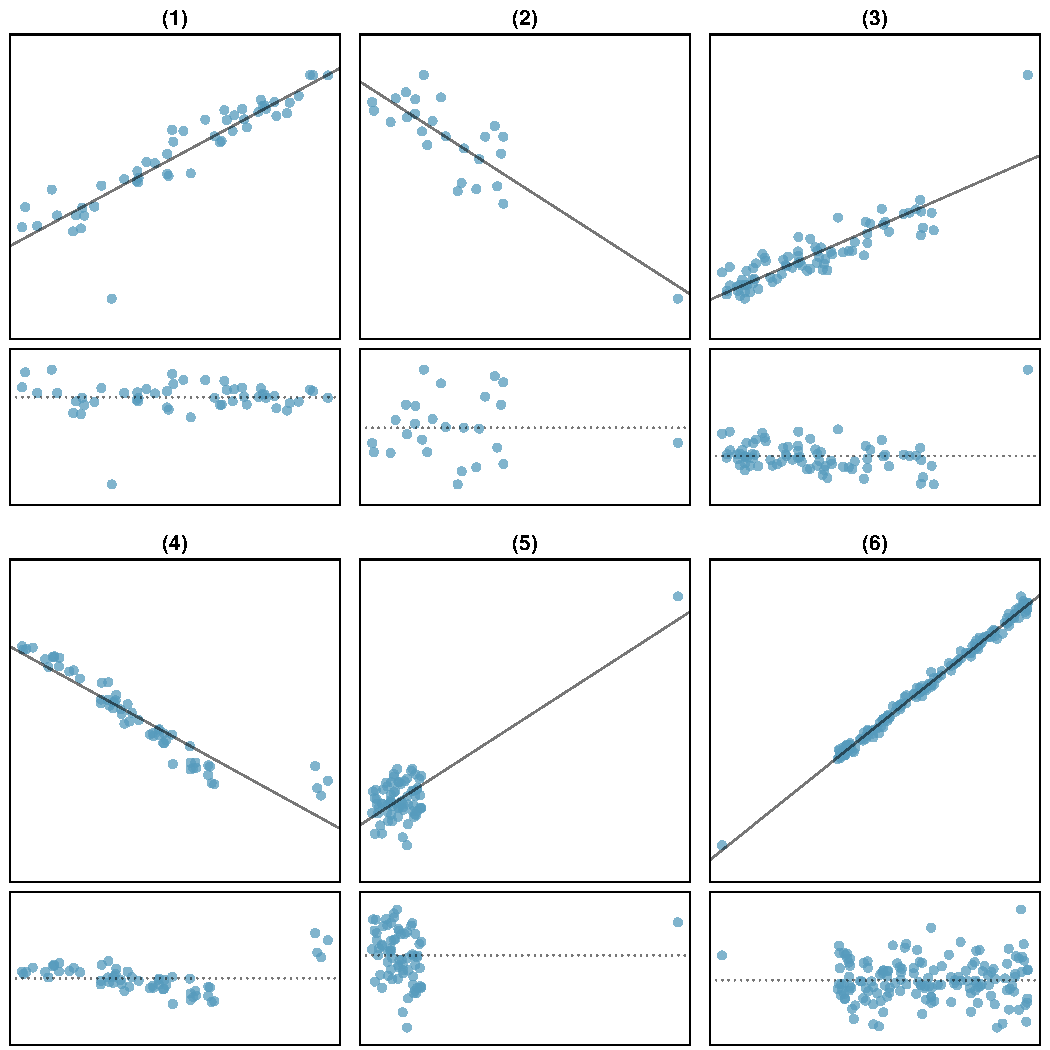
\includegraphics[width=\textwidth]{ch_regr_simple_linear/figures/outlierPlots/outlierPlots}
\caption{Six plots, each with a least squares line and residual plot. All data sets have at least one outlier.}
\label{outlierPlots}
\end{figure}


Examine the residual plots in Figure~\ref{outlierPlots}. You will probably find that there is some trend in the main clouds of (3) and (4). In these cases, the outliers influenced the slope of the least squares lines. In (5), data with no clear trend were assigned a line with a large trend simply due to one outlier (!).
 
 \begin{onebox}{Leverage}
Points that fall horizontally away from the center of the cloud tend to pull harder on the line, so we call them points with \term{high leverage}.\end{onebox}

Points that fall horizontally far from the line are points of high leverage; these points can strongly influence the slope of the least squares line. If one of these high leverage points does appear to actually invoke its influence on the slope of the line -- as in cases (3), (4), and (5) of Example~\ref{outlierPlotsExample} -- then we call it an \term{influential point}. Usually we can say a point is influential if, had we fitted the line without it, the influential point would have been unusually far from the least squares line.

It is tempting to remove outliers. Don't do this without a very good reason. Models that ignore exceptional (and interesting) cases often perform poorly. For instance, if a financial firm ignored the largest market swings -- the ``outliers'' --  they would soon go bankrupt by making poorly thought-out investments.

\begin{onebox}{Don't ignore outliers when fitting a final model}
{If there are outliers in the data, they should not be removed or ignored without a~good reason. Whatever final model is fit to the data would not be very helpful if it ignores the most exceptional cases.}
\end{onebox}

\begin{onebox}{Outliers for a categorical predictor with two levels}
{Be cautious about using a categorical predictor when one of the levels has very few observations. When this happens, those few observations become influential points.}
\end{onebox}



%%
\subsection{Categorical predictors with two levels (special topic)}
\label{categoricalPredictorsWithTwoLevels}

Categorical variables are also useful in predicting outcomes. Here we consider a categorical predictor with two levels (recall that a \emph{level} is the same as a \emph{category}). We'll consider Ebay auctions for a video game, \emph{Mario Kart} for the Nintendo Wii, where both the total price of the auction and the condition of the game were recorded.\footnote{These data were collected in Fall 2009 and may be found at \oiRedirect{textbook-openintro_org_stat}{openintro.org/stat}.} Here we want to predict total price based on game condition, which takes values \resp{used} and \resp{new}. A plot of the auction data is shown in Figure~\ref{marioKartNewUsed}.

\begin{figure}
\centering
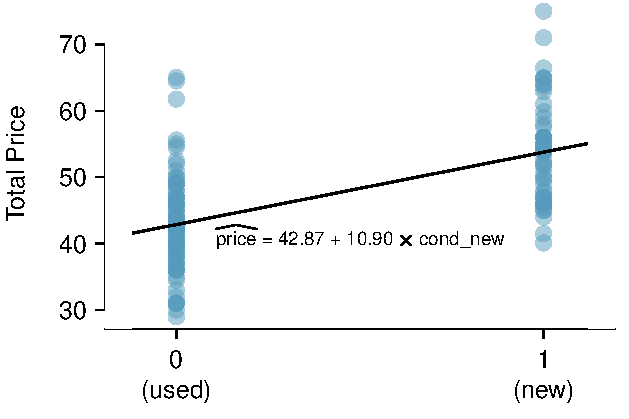
\includegraphics[width=0.6\textwidth]{ch_regr_simple_linear/figures/marioKartNewUsed/marioKartNewUsed}
\caption{Total auction prices for the video game \emph{Mario Kart}, divided into used ($x=0$) and new ($x=1$) condition games. The least squares regression line is also shown.}
\label{marioKartNewUsed}
\end{figure}

To incorporate the game condition variable into a regression equation, we must convert the categories into a numerical form. We will do so using an \term{indicator variable} called \var{cond\_\hspace{0.3mm}new}, which takes value 1 when the game is new and 0 when the game is used. Using this indicator variable, the linear model may be written as
\begin{align*}
\widehat{price} = \beta_0 + \beta_1 \times \text{\var{cond\_\hspace{0.3mm}new}}
\end{align*}
The fitted model is summarized in Table~\ref{marioKartNewUsedRegrSummary}, and the model with its parameter estimates is given as
\begin{align*}
\widehat{price} = 42.87 + 10.90 \times \text{\var{cond\_\hspace{0.3mm}new}}
\end{align*}
For categorical predictors with just two levels, the linearity assumption will always be satisfied. However, we must evaluate whether the residuals in each group are approximately normal and have approximately equal variance. As can be seen in Figure~\ref{marioKartNewUsed}, both of these conditions are reasonably satisfied by the auction data.

\begin{table}
\centering
\begin{tabular}{rrrrr}
  \hline
  \vspace{-3.7mm} & & & & \\
 & Estimate & Std. Error & t value & Pr($>$$|$t$|$) \\ 
  \hline
  \vspace{-3.6mm} & & & & \\
(Intercept) & 42.87 & 0.81 & 52.67 & 0.0000 \\ 
  cond\_\hspace{0.3mm}new & 10.90 & 1.26 & 8.66 & 0.0000 \\ 
   \hline
\end{tabular}
\caption{Least squares regression summary for the final auction price against the condition of the game.}
\label{marioKartNewUsedRegrSummary}
\end{table}

\begin{examplewrap}
\begin{nexample}{Interpret the two parameters estimated in the model for the price of \emph{Mario Kart} in eBay auctions.}
The intercept is the estimated price when \var{cond\_\hspace{0.3mm}new} takes value 0, i.e. when the game is in used condition. That is, the average selling price of a used version of the game is \$42.87.

The slope indicates that, on average, new games sell for about \$10.90 more than used games.
\end{nexample}
\end{examplewrap}

\begin{onebox}{Interpreting model estimates for categorical predictors.}
The estimated intercept is the value of the response variable for the first category (i.e. the category corresponding to an indicator value of 0). The estimated slope is the average change in the response variable between the two categories.\end{onebox}



%%
%%
\subsection*{Section summary}

\begin{itemize}
\item We define the \emph{best fit line} as the line that minimizes the sum of the squared residuals (errors) about the line.  That is, we find the line that minimizes $(y_1 - \hat{y}_1)^2 + (y_2-\hat{y}_2)^2+ \dots + (y_n-\hat{y}_n)^2=\sum{(y_i - \hat{y}_i)^2}$. We call this line the \term{least squares regression line}.

\item We write the least squares regression line in the form: $\hat{y} = b_0 + b_1x$,  and we can calculate $b_0$ and $b_1$ based on the summary statistics as follows:
\begin{eqnarray*}
b_1=r\frac{s_y}{s_x} \qquad \text{and} \qquad b_0=\bar{y} - b_1\bar{x}.
\end{eqnarray*}

\item $b_0$ and $b_1$ are point estimates for the parameters $\beta_0$ and $\beta_1$ in the true model, given by:  \mbox{$y=\beta_0+\beta_1x+\textit{error}$.}

\item \emph{Interpreting} the \term{y-intercept} and \term{slope} of a linear model
\begin{itemize}
\item The slope, $b_1$, describes the \emph{average} increase or decrease in the $y$ variable if the explanatory variable $x$ is one unit larger. 
\item The y-intercept, $b_0$, describes the average or predicted outcome of $y$ if $x=0$.  The linear model must be valid all the way to $x=0$ for this to make sense, which in many applications is not the case.
\end{itemize}

\item Two important considerations about the regression line
\begin{itemize}
\item  The regression line provides \textit{estimates} or \textit{predictions}, not actual values.  It is important to how large $s$, the standard deviation of the residuals, is, in order to know about how much error to expect in these predictions.
\item The regression line estimates are only reasonable within the domain of the data.  Predicting $y$ for $x$ values that are outside the domain, known as \term{extrapolation}, is unreliable and may produce ridiculous results.
\end{itemize}

\item Using $R^2$ to assess the fit of the model
\begin{itemize}
\item $R^2$, called \term{R-squared} or the \term{explained variance}, is a measure of how well the model explains or fits the data.
\item The $R^2$ of a linear model describes the \emph{proportion of variation} in the $y$ variable that is \emph{explained by} the regression line.
\item $R^2$ is always between 0 and 1, inclusive, or between 0\% and 100\%, inclusive.  The higher the value of $R^2$, the better the model ``fits" the data.  
\item $R^2$ applies to any type of model, not just a linear model, and can be used to compare the fit among various models.
\item The correlation coefficient $r = \pm\sqrt{R^2}$. The value of $R^2$ is always positive and cannot tell us the \emph{direction} of the association.  If finding $r$ based on $R^2$, make sure to use either the scatterplot or the slope of the regression line to determine the \emph{sign} of $r$.
\end{itemize}

\item When a residual plot of the data appears as a random cloud of points, a linear model is generally appropriate. If a residual plot of the data has any type of pattern, such as a $\cup$-shape, a linear model is not appropriate.

\item \term{Outliers} in regression are observations that fall far from the ``cloud" of points.

\item An \term{infuential point} is a point that has a big effect or pull on the slope of the regression line.  

\item Points that are outliers in the $x$ direction will have more pull on the slope of the regression line and are more likely to be influential points.

\item Outliers in the data should not be removed or ignored without a good reason; often these points  communicate important aspects about the association.
\end{itemize}




%__________________
\section[Inference for the slope of a regression line]{Inference for the slope of a regression line }
\label{inferenceForLinearRegression}

\sectionintro{
\begin{itemize}
\item Is the unemployment rate a significant linear predictor for the loss of the President's party in the House of Representatives?

\item How well does the price of textbooks at the UCLA Bookstore predict the price on Amazon? 

\end{itemize}

\subsection*{Learning objectives}
\begin{enumerate}
\item Recognize that the sample slope is a point estimate and has an associated standard error.

\item Be able to read the results of computer regression output and identify the quantities needed for inference for the slope of the regression line, specifically the sample slope, the $SE$ of the slope, and the degrees of freedom.

\item State and verify whether or not the conditions for inference on the slope of the regression line based using the $t$-distribution are met.

\item Carry out a complete confidence interval procedure for the slope of the regression line.  


\item Carry out a complete hypothesis test for the slope of the regression line.

\item Distinguish between when to use the linear regression $t$-test and when to use the matched pairs $t$-test.
\end{enumerate}
}

\subsection{The role of inference for regression parameters}
Previously, we looked at a set of paired data involving the price of textbooks for UCLA courses at the UCLA Bookstore and on Amazon.  By carrying out a one sample $t$-test on the paired differences, we found that on average, prices are higher at the UCLA Bookstore.  

What if we are interested in estimating the change in price of  textbooks at the UCLA Bookstore relative to the change in price on Amazon?  This sounds like a slope, so we really we are interested in estimating the slope.  


Linear regression assumes that the relationship between two variables, $x$ and $y$, can be modeled by a straight line.  The equation for the true or population regression line can be written as
\begin{eqnarray*}
y = \beta_0 + \beta_1x +\epsilon
\end{eqnarray*}
Here, $\beta_0$ and $\beta_1$ represent two model parameters\index{parameter}, namely the $y$-intercept and the slope of the true or population regression line. ($\beta$ is the Greek letter \emph{beta}\index{Greek!beta@beta ($\beta$)}. This use of $\beta$ has nothing to do with the $\beta$ we used to describe the probability of a Type~II Error.) The error is represented by $\varepsilon$
(the Greek letter \emph{epsilon}\index{Greek!epsilon@epsilon ($\varepsilon$)}).
The parameters are estimated using data.  Now when we look at the equation of the regression line calculated from a particular data set:
\begin{align*}
\hat{y} =& b_0 + b_1x 
\end{align*}
we can see that $b_0$ and $b_1$ are point estimates for $\beta_0$ and $\beta_1$, respectively.  
In this case, the regression equation for predicting family aid based on income is:
\begin{align*}
\hat{y} = 1.86 + 1.03x
\end{align*}
The sample slope, 1.03, is our best estimate for the true slope, but there is variability in this estimate since it is based on a sample.  A different sample would produce a somewhat different estimate of the slope.  The standard error of the slope tells us the typical variation in the sample slope and the typical error in using the sample slope to estimate the true slope.  

We would like to construct a 95\% confidence interval for $\beta_1$, the true slope of the regression line. As with means, inference for the slope of a regression line is based on the $t$-distribution.

\begin{onebox}
{Inference for the slope of a regression line}
Inference for the slope of a regression line is based on the $t$-distribution with $n-2$ degrees of freedom, where $n$ is the number of paired observations.
\end{onebox}

The point estimate for the slope and standard error of the estimate have already been encountered in regression output.  Once we verify that conditions for using the $t$-distribution are met, we will be able to construct the confidence interval using a critical value $t^{\star}$ based on $n-2$ degrees of freedom.

%%
\subsection{Conditions for the least squares line}

Conditions for inference in the context of regression can be more complicated than when dealing with means or proportions.  

Inference for parameters of a regression line involves the following assumptions:
\begin{description}
\setlength{\itemsep}{0mm}
\item[Linearity.] The true relationship between the two variables follows a linear trend.  We see if this is reasonable by checking whether the data follows a linear trend.  If there is a nonlinear trend (e.g. left panel of Figure~\ref{whatCanGoWrongWithLinearModel}), an advanced regression method from another book or later course should be applied.
\item[Nearly normal residuals.] The residuals should be nearly normal.
When this assumption is found to be unreasonable, it is usually because of outliers or concerns about influential points.  An example which suggestions non-normal residuals is shown in the second panel of Figure~\ref{whatCanGoWrongWithLinearModel}.
\item[Constant variability.] The variability of points around the true least squares line is constant for all values of $x$. An example of non-constant variability is shown in the third panel of Figure~\ref{whatCanGoWrongWithLinearModel}.
\item[Independent.] The observations are independent of one other.  The observations can be considered independent when they are collected from a random sample or randomized experiment.  Be careful of data collected sequentially in what is called a \term{time series}.  An example of data collected in such a fashion is shown in the fourth panel of Figure~\ref{whatCanGoWrongWithLinearModel}.
\end{description}

\begin{figure}
\centering
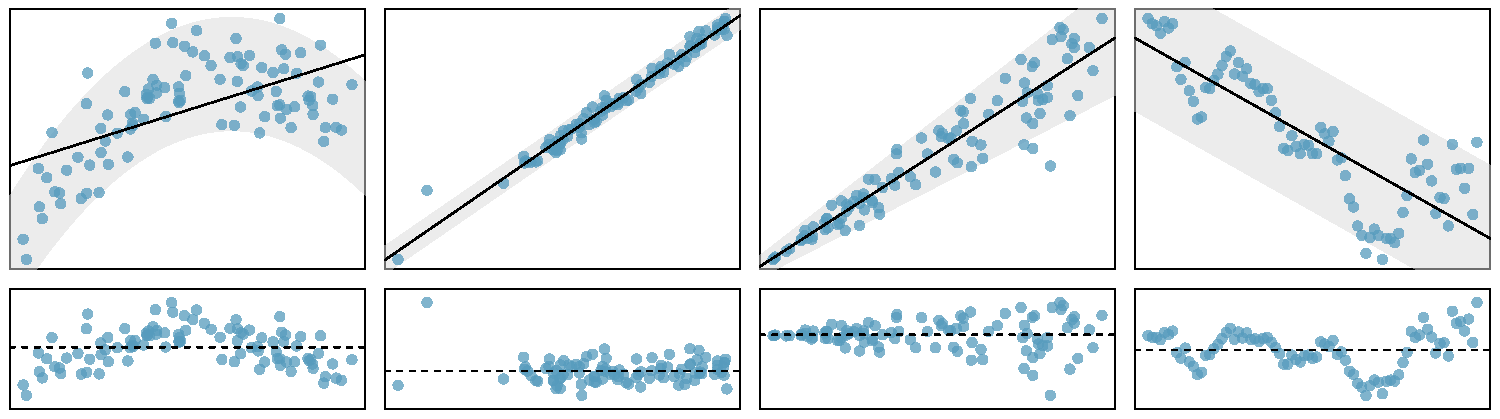
\includegraphics[width=\textwidth]{ch_regr_simple_linear/figures/whatCanGoWrongWithLinearModel/whatCanGoWrongWithLinearModel}
\caption{Four examples showing when the methods in this chapter are insufficient to apply to the data. In the left panel, a straight line does not fit the data. In the second panel, there are outliers; two points on the left are relatively distant from the rest of the data, and one of these points is very far away from the line. In the third panel, the variability of the data around the line increases with larger values of $x$. In the last panel, a time series data set is shown, where successive observations are highly correlated.}
\label{whatCanGoWrongWithLinearModel}
\end{figure}

We see in Figure~{whatCanGoWrongWithLinearModel}, that patters in the residual plot suggest that the assumptions for regression inference are not met.  In fact, identifying nonlinear trends in the data, outliers, and non-constant variability in the residuals are often easier to detect in a residual plot than in a scatter plot.  

We note that the second assumption regarding nearly normal residuals is particularly difficult to assess when the sample size is small.  We can make a graph, such as a histogram, of the residuals, but we cannot expect a small data set to be nearly normal.  All we can do is to look for excessive skew or outliers.  Outliers and influential points in the data can be seen from the residual plot as well as from a histogram of the residuals.

\begin{onebox}{Conditions for inference on the slope of a regression line}
\begin{enumerate}
\item The data is collected from a random sample or randomized experiment.
\item The residual plot appears as a random cloud of points and does not have any patters or significant outliers that would suggest that the linearity, nearly normal residuals, constant variability or independence assumptions are unreasonable.  
\end{enumerate}
\end{onebox} 

\subsection{Constructing a confidence interval for the slope of a regression line}

We would like to construct a confidence interval for the true slope of the regression line for predicting textbook price at the UCLA Bookstore based on the textbook price on Amazon.  Consider the scatter plot and corresponding residual plot.  Do conditions seem to be satisfied?

We recall that textbooks were randomly chosen, so we will consider the observations independent.  Also, the residual plot shows no pattern in the residuals, indicating that a linear model is appropriate.  

We are now ready to calculate the 95\% confidence interval.  

\begin{examplewrap}
\begin{nexample}
{Construct a 95\% confidence interval for the slope of the regression line for predicting a textbook's price at the UCLA Boostore based on the textbook's price on Amazon.}
As usual, the confidence interval will take the form:  
\begin{align*}
\text{point estimate} \pm \text{critical value}\times SE \text{ of estimate}
\end{align*}
The point estimate for the true slope is the sample slope of 1.03.  The standard error of the slope can be read from the table as 0.030.  Note that we do not need to divide 0.030 by the square root of $n$ or do any further calculations on 0.030; 0.030 \emph{is} the $SE$ of the sample slope.  Here $n=68$, so $df=68-2=66$.  Rounding down to row $df=60$ with confidence level =95\%, we estimate the critical value $t^{\star}=2.000$.  The confidence interval is calculated as:
\begin{align*}
1.03 \ \pm \ & 2.000\times 0.030 \qquad df = 66 \\
=(0.97&,\ 1.09 )
\end{align*}
\end{nexample}
\end{examplewrap}

\begin{examplewrap}
\begin{nexample}
{Intepret the confidence interval in context.  What can we conclude?}
We are 95\% confident that the true slope, that is the true increase in textbook price at the UCLA Bookstore for each dollar increase on Amazon is between \$0.97 and \$1.09.  Because the entire interval is positive, we have evidence that the true slope is greater than 0, that is, that there is a positive linear relationship between textbook price on Amazon and at the UCLA Bookstore.
\end{nexample}
\end{examplewrap}

\begin{onebox}{Constructing a confidence interval for the slope of regression line}
To carry out a complete confidence interval procedure to estimate the true slope $\beta_1$ of a regression line,
\\
\\
\inferencestep{Identify} Identify the parameter and the confidence level, C\%.\vspace{-1mm}
\begin{itemize} 
\item[] The parameter will be a population slope, e.g. the true slope of the regression line relating air quality index to average rainfall per year for each city in the United States.  
\end{itemize}
\inferencestep{Choose} Choose the correct interval procedure and identify it by name. \vspace{-1mm}
\begin{itemize}
\item[] Here we use choose the \term{Linear regression $t$-interval for the slope} .
\end{itemize}
\inferencestep{Check} Check conditions for using a $t$-interval for the slope.\vspace{-1mm}
\begin{itemize}
\setlength{\itemsep}{0mm}
\item[] 1.  Data come from a random sample or randomized experiment.
\item[] 2.  The residual plot shows no pattern implying that a linear model is reasonable. \item[] \quad \ (More specifically, the residuals should be independent, nearly normal, and have
\item [] \quad \  constant standard deviation).
\end{itemize}
\inferencestep{Calculate} Calculate the confidence interval and record it in interval form.
\begin{itemize}
\item[] $\text{point estimate}\ \pm\ t^{\star} \times SE\ \text{of estimate}$, \quad $df = n - 2$
\begin{itemize}											
\item[] point estimate: the sample slope $b_1$
\item[] $SE$ of estimate: $SE$ of slope (find using computer output)
\item[] $t^{\star}$: use a $t$-table at row $df = n-2$ and confidence level C\%
\end{itemize}
\item[] (\underline{\ \ \ \ \ }, \underline{\ \ \ \ \ })
\end{itemize}
\inferencestep{Conclude}  Interpret the interval and, if applicable, draw a conclusion in context.\vspace{-1mm}
\begin{itemize}
\item[] We are C\%  confident that the true \emph{slope} of the regression line relating [y] to [x] is between \underline{\ \ \ \ \ } and \underline{\ \ \ \ \ }. If applicable, draw a conclusion based on whether the interval is entirely above, is entirely below, or contains the value 0. 
\end{itemize}
\end{onebox}

\begin{examplewrap}
\begin{nexample}{
The regression summary below shows statistical software output from fitting the least squares regression line for predicting gift aid based on family income at Elmhurst College.  The scatterplot was shown in Figure~\ref{elmhurstScatterWLSROnly}. 
\\
\\
\texttt{Predictor \ \ \ \ \ \ \ Coef \ \ \ \ \ \ \ SE Coef \ \ T \ \ \ \ \ \ \ P} \\
\texttt{Constant \ \ \ \ \ \ \ \  24.31933 \ \ \ 1.29145 \ \ 18.831 \ \ < 2e-16} \\
\texttt{family\_income\ \ \ \ -0.04307 \ \ \ 0.01081 \ \ -3.985 \ \ 0.000229} \\

\texttt{S = 4.783\ \ \ \ R-Sq = 24.86\% \ \ \ R-Sq(adj) = 23.29\%}
%\label{rOutputForIncomeAidLSRLineInInferenceSection}
\\
\\
Construct a 95\% confidence interval for the slope of the regression line.  Is there convincing evidence that there is a negative, linear relationship between family income and gift aid? Use the five step framework described previously to organize your work.}
\begin{description}
\item[\inferencestep{Identify}] The parameter of interest is the true slope of the line for predicting gift aid based on family income.  We want to estimate this at the 95\% confidence level.  
\item[\inferencestep{Choose}] Because the parameter to be estimated is the slope of a regression line, we will use the Linear regression $t$-interval for the slope.
\item[\inferencestep{Check}] 
\item[\inferencestep{Calculate}]  We will calculate the interval:
\begin{align*}
\text{point estimate}\ \pm\ t^{\star} \times SE\ \text{of estimate}
\end{align*}
We read the sample slope and the corresponding $SE$ from the table.
\\
\\
The point estimate is the sample slope: $b_1 = -0.04307$\\
\\
The $SE$ of the sample slope is 0.01081.  
\\
\\
Degrees of freedom $df=n-2=50-2=48$.
\\
\\
As before, we find the critical value $t^{\star}$ using a $t$-table (the $t^{\star}$ value is not the same as the $T$-statistic for the hypothesis test).   Using the $t$-table at row $df = 40$ (round down since 48 is not on the table) and confidence level 95\%, we get $t^{\star}=2.021$.  
\\
\\
So the 95\% confidence interval is given by:
\begin{align*}
-0.04307 \ \pm\  &2.021\times  0.01081 
=()
\end{align*}
\item[\inferencestep{Conclude}]  We are 95\% confident that the true slope, that is, the true average \emph{decrease} in gift aid for each additional thousand dollars in family income, falls between and .  Because the interval is entirely below 0, we do have evidence of a negative linear association between the variables.  
\end{description}


\end{nexample}
\end{examplewrap}
\textA{\newpage}

\subsection{Calculator: Linear regression $t$-interval for the slope}
We will rely on regression output from statistical software when constructing confidence intervals for the slope of a regression line.  We include calculator instructions here simply for completion.

\begin{onebox}{\videohref{ti84_regression_t_confint} TI-84: $t$-interval for $\beta_1$}
\label{LinRegint}
Use \calctext{STAT}, \calctext{TESTS}, \calctext{LinRegTInt}.
\begin{enumerate}
\setlength{\itemsep}{0mm}
\item Choose \calctext{STAT}.
\item Right arrow to \calctext{TESTS}.
\item Down arrow and choose \calctext{G:} \calctext{LinRegTInt}.\vspace{-1.5mm}
  \begin{itemize}
  \item This test is not built into the TI-83.
  \end{itemize}
\item Let \calctext{Xlist} be \calctext{L1} and \calctext{Ylist} be \calctext{L2}. (Don't forget to enter the $x$ and $y$ values in \calctext{L1} and \calctext{L2} before doing this interval.)
\item Let \calctext{Freq} be \calctext{1}.
\item Enter the desired confidence level.
\item Leave \calctext{RegEQ} blank.
\item Choose \calctext{Calculate} and hit \calcbutton{ENTER}, which returns: \\[1mm]
\begin{tabular}{l l}
\calctext{(\underline{\ \ },\underline{\ \ })} & the confidence interval \\
\calctext{b} & $b_1$, the slope of best fit line of the sample data \\
\calctext{df} &degrees of freedom associated with this confidence interval \\
\calctext{s} & standard deviation of the residuals (not the same as $SE$ of the slope) \\
\calctext{a} & $b_0$, the y-intercept of the best fit line of the sample data \\
$\calctextmath{r^2}$ & $R^2$, the explained variance \\
\calctext{r} & $r$, the correlation coefficient \\
\end{tabular}
\end{enumerate}
\end{onebox}




\Comment{rename with something more specific? hypothesis testing and ci for the slope?}
%%
\subsection{Midterm elections and unemployment}

\index{data!midterm elections|(}

Elections for members of the United States House of Representatives occur every two years, coinciding every four years with the U.S. Presidential election. The set of House elections occurring during the middle of a Presidential term are called \indexthis{midterm elections}{midterm election}. In America's two-party system, one political theory suggests the higher the unemployment rate, the worse the President's party will do in the midterm elections.

To assess the validity of this claim, we can compile historical data and look for a connection. We consider every midterm election from 1898 to 2018, with the exception of those elections during the Great Depression. Figure~\ref{unemploymentAndChangeInHouse} shows these data and the least-squares regression line: \vspace{-2mm}
\begin{align*}
&\text{\% change in House seats for President's party}  \\
&\qquad\qquad= -7.36 - 0.89\times \text{(unemployment rate)}
\end{align*}
We consider the percent change in the number of seats of the President's party (e.g. percent change in the number of seats for Republicans in 2018) against the unemployment rate.

Examining the data, there are no clear deviations from linearity, the constant variance condition, or in the normality of residuals (though we don't examine a normal probability plot here). While the data are collected sequentially, a separate analysis was used to check for any apparent correlation between successive observations; no such correlation was found.

\begin{figure}
\centering
 \href{\oiRedirectUrl{tableau_scatter_change_in_house_seats}}{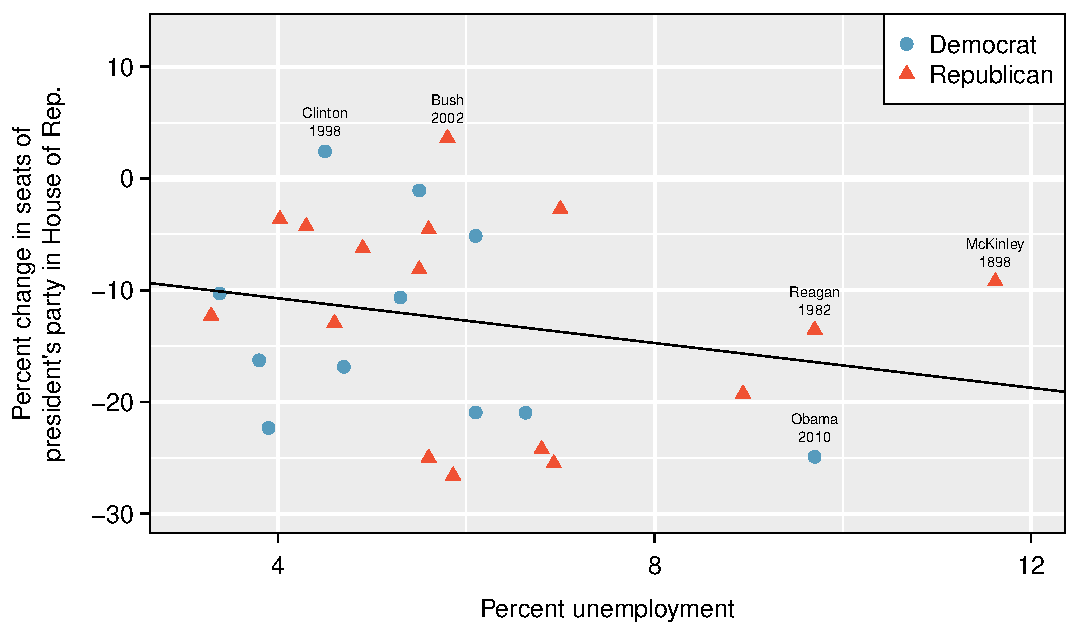
\includegraphics[width=\textwidth]{ch_regr_simple_linear/figures/unemploymentAndChangeInHouse/unemploymentAndChangeInHouse}}
\caption{The percent change in House seats for the President's party in each election from 1898 to 2018 plotted against the unemployment rate. The two points for the Great Depression have been removed, and a least squares regression line has been fit to the data.}
\label{unemploymentAndChangeInHouse}
\end{figure}

\begin{exercisewrap}
\begin{nexercise}
The data for the Great Depression (1934 and 1938) were removed because the unemployment rate was 21\% and 18\%, respectively. Do you agree that they should be removed for this investigation? Why or why not?\footnotemark 
\end{nexercise}
\end{exercisewrap}
\footnotetext{We will provide two considerations. Each of these points would have very high leverage on any least-squares regression line, and years with such high unemployment may not help us understand what would happen in other years where the unemployment is only modestly high. On the other hand, these are exceptional cases, and we would be discarding important information if we exclude them from a final analysis.}

\textA{\newpage}

There is a negative slope in the line shown in Figure~\ref{unemploymentAndChangeInHouse}. However, this slope (and the y-intercept) are only estimates of the parameter values. We might wonder, is this convincing evidence that the ``true'' linear model has a negative? That is, do the data provide strong evidence that the political theory is accurate?  We can frame this investigation as a statistical hypothesis test:
\begin{itemize}
\item[$H_0$:] $\beta_1 = 0$. The true linear model has slope zero.
\item[$H_A$:] $\beta_1 < 0$. The true linear model has a slope less than zero. The higher the unemployment, the greater the loss for the President's party in the House of Representatives.
\end{itemize}
We would reject $H_0$ in favor of $H_A$ if the data provide strong evidence that the true slope parameter is less than zero. To assess the hypotheses, we identify a standard error for the estimate, compute an appropriate test statistic, and identify the p-value.


%%
\subsection{Understanding regression output from software}
\label{testStatisticForTheSlope}

Just like other point estimates we have seen before, we can compute a standard error and test statistic for $b_1$. We will generally label the test statistic using a $T$, since it follows the $t$-distribution.

\begin{onebox}{Hypothesis tests on the slope of the regression line}
Use a $t$-test with $n - 2$ degrees of freedom when performing a hypothesis test on the slope of a regression line.\end{onebox}


We will rely on statistical software to compute the standard error and leave the explanation of how this standard error is determined to a second or third statistics course. The table below shows software output for the least squares regression line in Figure~\ref{unemploymentAndChangeInHouse}. The row labeled \emph{unemp} represents the information for the slope, which is the coefficient of the unemployment variable.

\begin{onebox}{\texttt{The regression output}} 


\texttt{Predictor \ \ \ \ \ Coef \ \ SE Coef \ \ \ \ \ \ T \ \ \ \ \ \ \ P} \\
\texttt{Constant \ \ \ -7.3644 \ \ \ 5.1553 \ \ -1.43 \ \ 0..1646} \\
\texttt{unemp \ \ \ \ \ \ -0.8897 \ \ \ 0.8350 \ \ -1.07 \ \ 0.2961} \\

\texttt{S = 9.624\ \ \ \ R-Sq = 0.03\% \ \ \ R-Sq(adj) = -3.7\%}
\end{onebox}
\label{midtermElectionUnemploymentRRegressionOutput}


\begin{examplewrap}
\begin{nexample}{What do the first column of numbers in the regression summary represent?}
The entries in the first column represent the least squares estimates for the $y$-intercept and slope, $b_0$ and $b_1$ respectively.  Using this information, we could write the equation
  for the least square regression line as
  \begin{align*}
  \hat{y} = -7.3644 - 0.8897 x
  \end{align*}
  where $y$ in this case represents the change in the number
  of seats for the president's party,
  and $x$ represents the unemployment rate.
\end{nexample}
\end{examplewrap}

We previously used a $T$ test statistic for hypothesis testing in the context of means. Regression is very similar. Here, the point estimate is the sample slope, $b_1=-0.8897$.  The $SE$ of the estimate is 0.8350, which is given in the second column, next to the estimate of $b_1$.  This $SE$ represents the typical error when using the sample slope to estimate the true slope.

The null value for the slope is 0, so we now have everything we need to compute the test statistic.  We have: 
\begin{align*}
T = \frac{\text{point estimate} - \text{null value}}{SE \text{ of estimate}} = \frac{-0.8897 - 0}{0.8350} = -1.07
\end{align*}
This value corresponds to the $T$ score reported in the regression output in the third column along the \emph{unemp} row.  

\begin{figure}
\centering
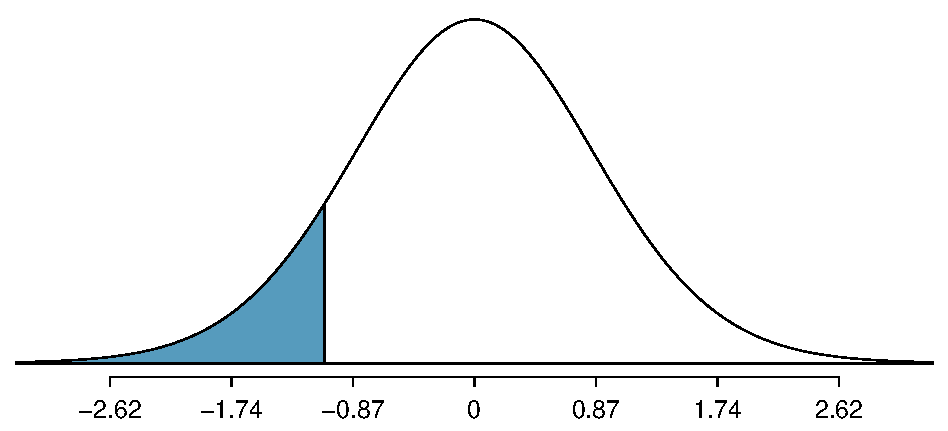
\includegraphics[width=0.82\textwidth]{ch_regr_simple_linear/figures/oneSidedTailForMidtermUnemploymentHT/oneSidedTailForMidtermUnemploymentHT}
\caption{The distribution shown here is the sampling distribution for $b_1$, if the null hypothesis was true. The shaded tail represents the p-value for the hypothesis test evaluating whether there is convincing evidence that higher unemployment corresponds to a greater loss of House seats for the President's party during a midterm election.}
\label{oneSidedTailForMidtermUnemploymentHT}
\end{figure}

\begin{examplewrap}
\begin{nexample}{In this example, the sample size $n=27$. Identify the degrees of freedom and p-value for the hypothesis test.}
The degrees of freedom for this test is $n-2$, or $df = 27-2 = 25$. We could use a table or a calculator to find the probability of a value less than -1.07 under the $t$-distribution with 25 degrees of freedom.  However, the two-side p-value is given in table, next to the corresponding $t$-statistic.  Because we have a one-sided alternate hypothesis, we take half of this.  The p-value for out test, then, is $\frac{0.2961}{2}=0.148$.  
\index{data!midterm elections|)}
\end{nexample}
\end{examplewrap}

Because the p-value is so large, we do not reject the null hypothesis. That is, the data do not provide convincing evidence that a higher unemployment rate is associated with a larger loss for the President's party in the House of Representatives in midterm elections.


\begin{onebox}{Inference for regression}
We usually rely on statistical software to identify point estimates and standard errors when carrying out inference on the slope of a regression line. After verifying conditions hold for fitting a line, we can use the methods learned in Section~\ref{oneSampleMeansWithTDistribution} for the $t$-distribution to create confidence intervals for regression parameters or to evaluate hypothesis tests.\end{onebox}

\begin{onebox}{Don't carelessly use the p-value from regression output}
{The last column in regression output often lists p-values for one particular hypothesis: a two-sided test where the null value is zero. If your test is one-sided and the point estimate is in the direction of $H_A$, then you can halve the software's p-value to get the one-tail area. If neither of these scenarios match your hypothesis test, be cautious about using the software output to obtain the p-value.}
\end{onebox}

\begin{onebox}{Always check conditions}
Do not blindly apply formulas or rely on regression output; always first look at a scatterplot or a residual plot.  If conditions for fitting the regression line are not met, the methods presented here should not be applied. 
\end{onebox}





%%

\begin{onebox}{Hypothesis test for the slope of regression line}
To carry out a complete hypothesis test to test the claim that there is no linear relationship between two numerical variables, i.e. that $\beta_1=0$, 
\\
\\
\inferencestep{Identify} Identify the hypotheses and the significance level, $\alpha$.\vspace{-1mm}
\begin{itemize}
\setlength{\itemsep}{0mm}
\item[] $H_0$: $\beta_1 = 0$  
\item[]  $H_A$: $\beta_1 \ne 0$;  \quad $H_A$: $\beta_1 > 0$; \quad or \quad $H_A$: $\beta_1 < 0$ 
\end{itemize} 
\inferencestep{Choose} Choose the correct test procedure and identify it by name. \vspace{-1mm}
\begin{itemize}
\item[] Here we choose the \term{Linear regression $t$-test for the slope}. 
\end{itemize}
 \inferencestep{Check} Check conditions for using a $t$-test for the slope.\vspace{-1mm}
\begin{itemize}
\setlength{\itemsep}{0mm}
\item[] 1.  Data come from a random sample or randomized experiment.
\item[] 2.  The residual plot shows no pattern implying that a linear model is reasonable. \item[] \quad \ (More specifically, the residuals should be independent, nearly normal, and have  
\item [] \quad \  constant standard deviation).
\end{itemize}
 \inferencestep{Calculate}  Calculate the $t$-statistic, $df$, and p-value.
\begin{itemize}
\item[] $T= \frac{\text{point estimate } - \text{ null value}}{SE \text{ of estimate}}$, \quad $df=n-2$
\begin{itemize}
\item[] point estimate: the sample slope $b_1$
\item[] $SE$ of estimate:  $SE$ of slope (find using computer output)
\item[] null value: 0
\end{itemize}
\item[] p-value = (based on the $t$-statistic, the $df$, and the direction of $H_A$)
\end{itemize}
 \inferencestep{Conclude} Compare the p-value to $\alpha$, and draw a conclusion in context. \vspace{-1mm}
\begin{itemize}
\item[] If the p-value is $< \alpha$, reject $H_0$; there is sufficient evidence that [$H_A$ in context]. 
\item[] If the p-value is $> \alpha$, do not reject $H_0$; there is not sufficient evidence that [$H_A$ in context].
\end{itemize}\end{onebox}


\begin{examplewrap}
\begin{nexample}{
The regression summary below shows statistical software output from fitting the least squares regression line for predicting gift aid based on family income at Elmhurst College.  The scatterplot was shown in Figure~\ref{elmhurstScatterWLSROnly}. 
\\
\\
\texttt{Predictor \ \ \ \ \ \ \ Coef \ \ \ \ \ \ \ SE Coef \ \ T \ \ \ \ \ \ \ P} \\
\texttt{Constant \ \ \ \ \ \ \ \  24.31933 \ \ \ 1.29145 \ \ 18.831 \ \ < 2e-16} \\
\texttt{family\_income\ \ \ \ -0.04307 \ \ \ 0.01081 \ \ -3.985 \ \ 0.000229} \\

\texttt{S = 4.783\ \ \ \ R-Sq = 24.86\% \ \ \ R-Sq(adj) = 23.29\%}
%\label{rOutputForIncomeAidLSRLineInInferenceSection}
\\
\\
Do these data provide convincing evidence that there is a negative, linear relationship between family income and gift aid?  Carry out a complete hypothesis test at the 0.05 significance level.  Use the five step framework described previously to organize your work.}

\begin{description}
\item[\inferencestep{Identify}]  We will test the following hypotheses at the $\alpha=0.05$ significance level.\\
$H_0$: $\beta_1 = 0$. There is no linear relationship.\\
$H_A$: $\beta_1 < 0$. There is a negative linear relationship.  
\\
\\
Here, $\beta_1$ is the slope of the true regression line for predicting gift aid from family income at Elmhurst College.
\item[\inferencestep{Choose}] Because the hypotheses are about the slope of a regression line, we choose the linear regression $t$-test for a slope.  
\item[\inferencestep{Check}]  
\item[ \inferencestep{Calculate} ]  We will calculate the test statistic, degrees of freedom, and the p-value.
\begin{align*}
T = \frac{\text{point estimate } - \text{ null value}}{SE \text{ of estimate}}
\end{align*}
We read the sample slope and the corresponding $SE$ from the table.
\\
\\
The point estimate is the sample slope: $b_1 = -0.04307$\\
\\
The $SE$ of the sample slope is 0.01081.  
\begin{align*}
T = \frac{-0.04307 - 0}{0.01081} = -3.985
\end{align*}
Because $H_A$ uses a less than sign ($<$), meaning that it is a lower-tail test, the \mbox{p-value} is the area to the \emph{left} of $t=-3.985$ under the $t$-distribution with $n-2=$ degrees of freedom.  The p-value = $\frac{1}{2}(0.000229)\approx 0.0001$.  
\item[\inferencestep{Conclude}]  The p-value of 0.0001 is $< 0.0.05$, so we reject $H_0$; there is sufficient evidence that there is negative linear relationship between family income and gift aid at Elmhurst College.  
\end{description}



\end{nexample}
\end{examplewrap}
\label{overallAidIncomeInformalAssessmentOfRegressionLineSlope}







\textA{\newpage}

%%
\subsection{Calculator: the linear regression $t$-test and $t$-interval}

When performing this type of inference, we generally make use of regression output that provides us with the necessary quantities: $b_1$ and $SE \text{ of } {b_1}$.  The calculator functions below require knowing all of the data and are, therefore, rarely used.  We describe them here for the sake of completion. 

\begin{onebox}{\videohref{ti84_regression_t_test} TI-83/84: Linear regression $t$-test on $\beta_1$}
\label{LinRegtest}
Use \calctext{STAT}, \calctext{TESTS}, \calctext{LinRegTTest}.
\begin{enumerate}
\setlength{\itemsep}{0mm}
\item Choose \calctext{STAT}.
\item Right arrow to \calctext{TESTS}.
\item Down arrow and choose \calctext{F:LinRegTTest}. (On TI-83 it is \calctext{E:LinRegTTest}).
\item Let \calctext{Xlist} be \calctext{L1} and \calctext{Ylist} be \calctext{L2}. (Don't forget to enter the $x$ and $y$ values in \calctext{L1} and \calctext{L2} before doing this test.)
\item Let \calctext{Freq} be \calctext{1}.
\item Choose $\calctextmath{\ne}$, $\calctextmath{<}$, or $\calctextmath{>}$ to correspond to $H_A$.
\item Leave \calctext{RegEQ} blank.
\item Choose \calctext{Calculate} and hit \calcbutton{ENTER}, which returns: \\[1mm]
\begin{tabular}{ll l ll}
\calctext{t} & t statistic &\quad&
	\calctext{b} & $b_1$, slope of the line \\
\calctext{p} & p-value &&
	\calctext{s} & st.~dev.~of the residuals \\
\calctext{df} & degrees of freedom for the test &&
	$\calctextmath{r^2}$ & $R^2$, explained variance \\
\calctext{a} & $b_0$, y-intercept of the line &&
	\calctext{r} & $r$, correlation coefficient
\end{tabular}
\end{enumerate}
\end{onebox} 

\begin{onebox}{\videohref{casio_regression_t_test} Casio fx-9750GII: Linear regression $t$-test on $\beta_1$}
\begin{enumerate}
\setlength{\itemsep}{0mm}
\item Navigate to \calctext{STAT} (\calcbutton{MENU} button, then hit the \calcbutton{2} button or select \calctext{STAT}).
\item Enter your data into 2 lists.
\item Select \calctext{TEST} (\calcbutton{F3}), \calctext{t} (\calcbutton{F2}), and \calctext{REG} (\calcbutton{F3}).
\item If needed, update the sidedness of the test and the \calctext{XList} and \calctext{YList} lists. The \calctext{Freq} should be set to \calctext{1}.
\item Hit \calcbutton{EXE}, which returns: \\[1mm]
\begin{tabular}{ll l ll}
\calctext{t} & t statistic &\quad&
	\calctext{b} & $b_1$, slope of the line \\
\calctext{p} & p-value &&
	\calctext{s} & st.~dev.~of the residuals \\
\calctext{df} & degrees of freedom for the test &&
	\calctext{r} & $r$, correlation coefficient \\
\calctext{a} & $b_0$, y-intercept of the line &&
	$\calctextmath{r^2}$ & $R^2$, explained variance
\end{tabular}
\end{enumerate}
\end{onebox} 

\begin{examplewrap}
\begin{nexample}
{Why does the calculator test include the symbol $\rho$ when choosing the direction of the alternate hypothesis?}
Recall that $b_1=r\frac{s_y}{s_x}$.  If the slope of the true regression line is zero, the population correlation coefficient must also be zero.  The linear regression test for $\beta_1=0$ is equivalent, then, to a test for the population correlation coefficient $\rho=0$.
\end{nexample}
\end{examplewrap}




\textA{\newpage}
%%
\subsection*{Section summary}

\noindent In Chapter 6, we used a $\chi^2$ test of independence to test for association between two categorical variables.  In this section, we test for association/correlation between two numerical variables.
\begin{itemize}
\item We use the sample slope $b_1$ as a \emph{point estimate} for the population slope $\beta_1$.  The population slope is the true increase/decrease in $y$ for each unit increase in $x$.  If the population slope is 0, there is no linear relationship between the two variables.  
\item Under certain assumptions, the sampling distribution of $b_1$ is \emph{normal} and the distribution of the standardized test statistic using the sample standard deviation of the residuals follows a \term{t-distribution} with $n-2$ degrees of freedom.

\item When there is $(x, y)$ data and the parameter of interest is the true slope of a regression line, e.g. the true slope of the regression line relating air quality index to average rainfall per year for each city in the United States:
\begin{itemize}
\item Estimate $\beta_1$ at the C\% confidence level using a \term{Linear regression $\mathbf{t}$-interval} .
\item Test $H_0$: $\beta_1=0$ at the $\alpha$ significance level using a \term{Linear regression $\mathbf{t}$-test}.
\end{itemize}
\item The conditions for the linear regression $t$-interval and $t$-test for the slope are the same.
\begin{itemize}
\setlength{\itemsep}{0mm}
\item[1.] Data come from a random sample or randomized experiment.
\item[2.] The residual plot shows no pattern implying that a linear model is reasonable. \item[] (Technically, the residuals should be independent, nearly normal, and have constant standard deviation.)
\end{itemize}
\item The confidence interval and test statistic are calculated as follows:   
\begin{itemize}
\item[] Confidence interval:\ \  $\text{point estimate}\ \pm\ t^{\star} \times SE\ \text{of estimate}$, or
\item[] Test statistic:  $T = \frac{\text{point estimate } - \text{ null value}}{SE\ \text{of estimate}}$ \ and p-value
\begin{itemize}
\item[] point estimate:  the sample slope $b_1$
\item[] $SE$ of estimate:  $SE$ of slope (find using computer output)
\item[] $df = n-2$
\end{itemize}
\end{itemize}


\item If the confidence interval for the slope of the population regression line estimates the true average increase in the $y$-variable for each unit increase in the $x$-variable.

\item The linear regression $t$-test and the matched pairs $t$-test both involve \emph{paired}, numerical data.  However, the linear regression $t$-test for the slope asks if the two variables have a linear \emph{relationship}, specifically if the \emph{slope} of the population regression line is 0.  The matched pairs $t$-test, on the other hand, asks if the two variables are in some way the \emph{same}, specifically if the \emph{mean} of the population differences is 0.  
\end{itemize}

%%________________________________
\section{Transformations for nonlinear data}

\sectionintro{

%%
\subsection*{Learning objectives}
\begin{enumerate}
\item Recognize that data can often be transformed to produce a linear relationship and that this transformation often involves log (or ln) of the $y$-values and sometimes log (or ln) of the $x$-values.

\item Use residual plots to assess whether a linear model for transformed data is reasonable.
\end{enumerate}
}

%%
\subsection{Untransformed}

\begin{examplewrap}
\begin{nexample}{Consider the scatterplot and residual plot in Figure~\ref{NeedsTransform-PreTransform}. The regression output is also provided.  Would a linear model be a good model for the data shown?}
First, we can note the $R^2$ value is fairly large.  However, this alone does not mean that the model is good.  Another model might be much better.  When assessing the appropriateness of a linear model, we should look at the residual plot.  The U pattern in the residual plot tells us the original data is curved. If we inspect the two plots, we can see that for small and large values of $x$ we systematically underestimate $y$, whereas for middle values of $x$, we systematically overestimate $y$.  Because of this, the model is not appropriate, and we should not carry out a linear regression $t$-test for the slope because the conditions for inference are not met.  However, we might be able to use a transformation to linearize the data.
\end{nexample}
\end{examplewrap}

\begin{figure}
   \centering
   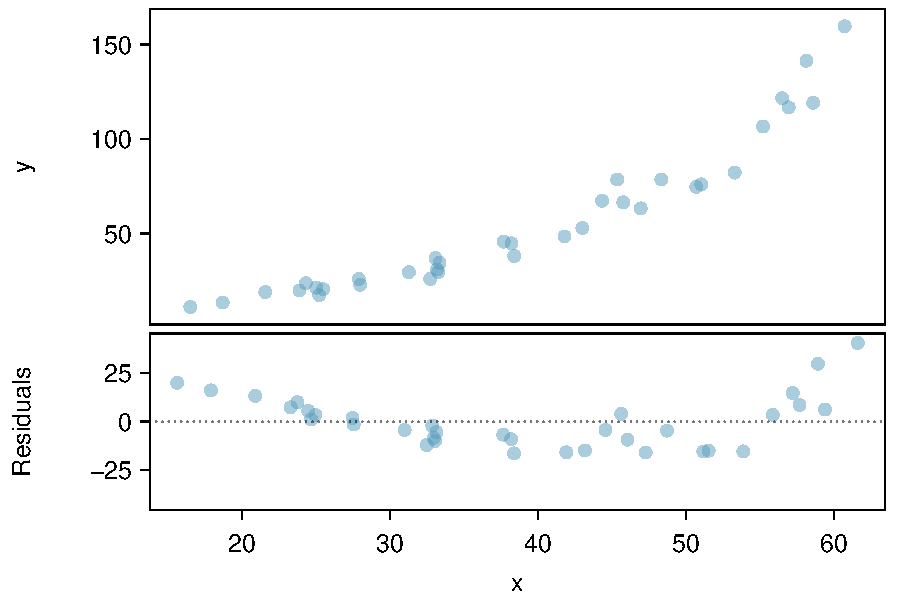
\includegraphics[width=0.7\textwidth]{ch_regr_simple_linear/figures/NeedsTransform/NeedsTransform-PreTransform}
   \caption{Variable $y$ is plotted against $x$. A nonlinear relationship is evident by the ``U'' shown in the residual plot. The curvature is also visible in the original plot.}
   \label{NeedsTransform-PreTransform}
\end{figure}


\begin{onebox}{\texttt{The regression equation is}} \\

\texttt{y = -52.3564 + 2.7842 x} \\

\texttt{Predictor \ \ \ \ \ \ Coef \ \ SE Coef \ \ \ \ \ \ \ \ T \ \ \ \ \ \ \ \ \ P} \\
\texttt{Constant \ \ \ -52.3564 \ \ \ 7.2757 \ \ \ -7.196 \ \ \ \ \ 3e-08} \\
\texttt{x \ \ \ \ \ \ \ \ \ \ \ \ 2.7842 \ \ \ 0.1768 \ \ \ 15.752 \ \ \ < 2e-16} \\

\texttt{S = 13.76\ \ \ \ R-Sq = 88.26\% \ \ \ R-Sq(adj) = 87.91\%}\end{onebox}


%%
\subsection{Transformed}

Regression analysis is easier to perform on linear data.  When data are nonlinear, we sometimes \term{transform} the data in a way that makes the resulting relationship linear.  The most common \term{transformation} is log (or ln) of the $y$ values. Sometimes we also apply a transformation to the $x$ values.  We generally use the residuals as a way to evaluate whether the transformed data are more linear. If so, we can say that a better model has been found.


\begin{examplewrap}
\begin{nexample}{Using the regression output for the transformed data, write the new linear regression equation}
$\widehat{log(y)} = 1.723 +0.053 x$
\end{nexample}
\end{examplewrap}

\begin{figure}
   \centering
   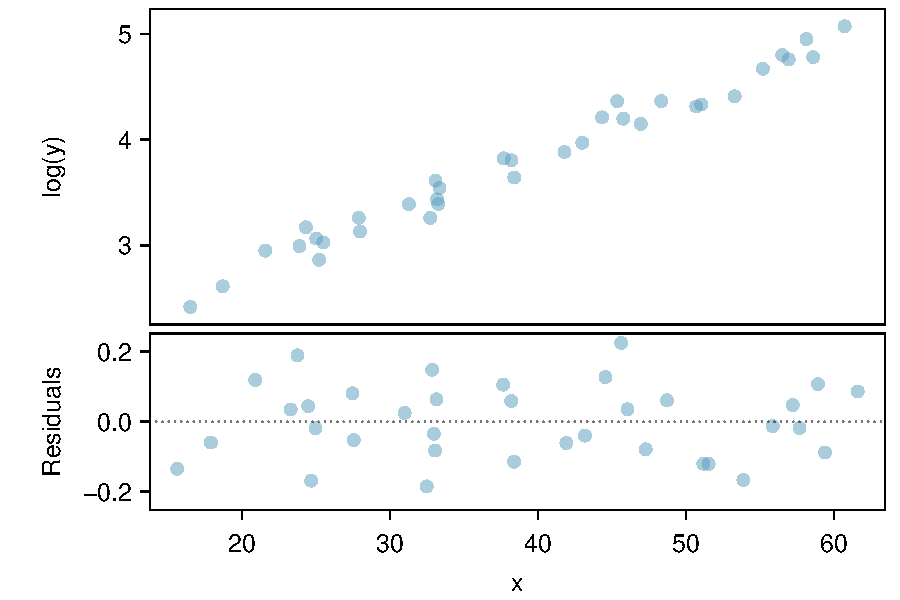
\includegraphics[width=0.7\textwidth]{ch_regr_simple_linear/figures/NeedsTransform/NeedsTransform-PostTransform}
   \caption{A plot of $\log(y)$ against $x$. The residuals don't show any evident patterns, which suggests the transformed data is well-fit by a linear model.}
   \label{NeedsTransform-PostTransform}
\end{figure}

\begin{onebox}{\texttt{The regression equation is}} \\

\texttt{log(y) = 1.722540 + 0.052985 x} \\

\texttt{Predictor \ \ \ \ \ \ \ \ Coef \ \ \ \ SE Coef \ \ \ \ \ \ \ T \ \ \ \ \ \ \ \ \ P} \\
\texttt{Constant \ \ \ \ \ 1.722540 \ \ \ 0.056731 \ \ \ 30.36 \ \ \ < 2e-16} \\
\texttt{x \ \ \ \ \ \ \ \ \ \ \ \ 0.052985 \ \ \ 0.001378 \ \ \ 38.45 \ \ \ < 2e-16} \\


\texttt{S = 0.1073\ \ \ \ R-Sq = 97.82\% \ \ \ R-Sq(adj) = 97.75\%}\end{onebox}

\begin{exercisewrap}
\begin{nexercise}Which of the following statements are true?  There may be more than one.\footnotemark 
\begin{enumerate}[(a)]
\item There is an apparent linear relationship between $x$ and $y$.
\item There is an apparent linear relationship between $x$ and $\widehat{log(y)}$.
\item The model provided by Regression I ($\hat{y} = -52.3564 + 2.7842 x$) yields a better~fit.
\item The model provided by Regression II ($\widehat{log(y)} = 1.723 +0.053 x$) yields a better~fit.
\end{enumerate}
\end{nexercise}
\end{exercisewrap}
\footnotetext{Part~(a) is \emph{false} since there is a nonlinear (curved) trend in the data. Part~(b) is true. Since the transformed data shows a stronger linear trend, it is a better fit, i.e. Part~(c) is \emph{false}, and Part~(d) is true.}

%%
%%
\subsection*{Section summary}
\begin{itemize}
\item Regression analysis is easier to perform on linear data. When data are nonlinear, we sometimes \term{transform} the data in a way that results in a linear relationship. The most common transformation is $log$ (or $ln$) of the $y$ values. Sometimes we also apply a transformation to the $x$ values. 

\item To assess the model, we look at the \textbf{residual plot} of the \emph{transformed} data.  If the residual plot of the original data has a pattern, but the residual plot of the transformed data has no pattern, a linear model for the transformed data is reasonable, and the transformed model provides a better fit than the simple linear model.

\end{itemize}



%_______________________
\section{Chapter Highlights}

\noindent This chapter focused on describing the linear association between two numerical variables and fitting a linear model.  
\begin{itemize}
\item The \term{correlation coefficient}, $r$, measures the strength and direction of the linear association between two variables.  However, $r$ alone cannot tell us whether data follow a linear trend or whether a linear model is appropriate.

\item The \term{explained variance}, $R^2$, measures the proportion of variation in the $y$ values explained by a given model.  Like $r$, $R^2$ alone cannot tell us whether data follow a linear trend or whether a linear model is appropriate.  

\item Every analysis should begin with \emph{graphing} the data using a \textbf{scatterplot} in order to see the association and any deviations from the trend (outliers or influential values).  A \textbf{residual plot} helps us better see patterns in the data.  

\item When the data show a linear trend, we fit a \textbf{least squares regression line} of the form: $\hat{y} = b_0+b_1x$, where $b_0$ is the $y$-intercept and $b_1$ is the slope.  It is important to be able to \emph{calculate} $b_0$ and $b_1$ using the summary statistics and to \emph{interpret} them in the context of the data.

\item A \textbf{residual}, $y-\hat{y}$, measures the error for an \emph{individual point}.  The \textbf{standard deviation of the residuals}, $s$, measures the typical size of the residuals.  

\item $\hat{y} = b_0+b_1x$ provides the best fit line for the \emph{observed data}.  To estimate or hypothesize about the true slope, first confirm that the residual plot has no pattern and that a linear model is reasonable, then use a \term{linear regression $t$-interval for the slope} or a \term{linear regression $t$-test for the slope} with $n-2$ degrees of freedom.
\end{itemize}
In this chapter we focused on simple linear models with one explanatory variable.  More complex methods of prediction, such as multiple regression (more than one explanatory variable) and nonlinear regression can be studied in a future course.


